\documentclass[review]{elsarticle}

\usepackage{lineno,hyperref}

\input merge_style.sty

\newcommand{\xl}[1]{\textbf{\textcolor{red}{(XL: #1)}}}
\newcommand{\ate}[1]{\textbf{\textcolor{blue}{(AE: #1)}}}% already was a command "\ae"
\newcommand{\ak}[1]{\textbf{\textcolor{green}{(AK: #1)}}}

\modulolinenumbers[5]

\journal{Journal of \LaTeX\ Templates}

%%%%%%%%%%%%%%%%%%%%%%%
%% Elsevier bibliography styles
%%%%%%%%%%%%%%%%%%%%%%%
%% To change the style, put a % in front of the second line of the current style and
%% remove the % from the second line of the style you would like to use.
%%%%%%%%%%%%%%%%%%%%%%%

%% Numbered
%\bibliographystyle{model1-num-names}

%% Numbered without titles
%\bibliographystyle{model1a-num-names}

%% Harvard
%\bibliographystyle{model2-names.bst}\biboptions{authoryear}

%% Vancouver numbered
%\usepackage{numcompress}\bibliographystyle{model3-num-names}

%% Vancouver name/year
%\usepackage{numcompress}\bibliographystyle{model4-names}\biboptions{authoryear}

%% APA style
\bibliographystyle{model5-names}\biboptions{authoryear}

%% AMA style
%\usepackage{numcompress}\bibliographystyle{model6-num-names}

%% `Elsevier LaTeX' style
% \bibliographystyle{elsarticle-num}
%%%%%%%%%%%%%%%%%%%%%%%

\begin{document}

\begin{frontmatter}

\title{Merge Search: a Matheuristic Framework for Combinatorial Optimisation Problems}
% \tnotetext[mytitlenote]{Fully documented templates are available in the elsarticle package on \href{http://www.ctan.org/tex-archive/macros/latex/contrib/elsarticle}{CTAN}.}

%% Group authors per affiliation:
\author[unsw]{Angus~Kenny}
\author[deak]{Dhananjay~Thiruvady}
\author[mon]{Davaatseren~Baatar}
\author[mon]{Andreas~T.~Ernst}
\author[rmit]{Xiaodong~Li}
\author[uq]{Mohan~Krishnamoorthy}
\author[bhp]{Gaurav~Singh}%

\address[unsw]{School of Engineering and Information Technology, University of New South Wales, Canberra ACT, Australia}
\address[deak]{School of Information Technology, Deakin University, Geelong VIC, Australia}
\address[mon]{School of Mathematics, Monash University, Clayton VIC, Australia}
% \address[4]{School of Mathematics, Monash University, Clayton VIC, Australia}
\address[rmit]{School of Computing Technologies, RMIT University, Melbourne VIC, Australia}
\address[uq]{School of Information Technology and Electrical Engineering, The University of Queensland, St Lucia QLD, Australia}
\address[bhp]{BHP, Perth WA, Australia}

\begin{abstract}
Exact methods are useful when solving combinatorial optimisation problems, although their time complexity is often high. Conversely, meta-heuristics are adept at finding feasible solutions in reasonable time, but their stochastic nature can make it hard to refine solutions effectively. To this end, a class of algorithms known as matheuristics was developed, which harness the strengths of both these methods.

This paper presents a matheuristic called merge search, an iterative decomposition algorithm which creates a reduced sub-problem by grouping variables that share common values across a population of solutions. Merge search can be thought of as a generalisation of crossover, from evolutionary algorithms; instead of combining two solutions to create a single offspring solution, the sub-space that is spanned by the entire population is searched for the optimal way to combine all solutions.

Merge search is applied to two very different NP-Hard problems: the constrained pit limit (CPIT) problem, from the field of open-pit mining; and the well-studied Steiner tree problem in graphs (STPG). The CPIT results are used to show the effectiveness of merge search, improving the best-known bounds in two of the six instances tested; while the STPG results demonstrate the versatility of this method. 
\end{abstract}

\begin{keyword}
\texttt{elsarticle.cls}\sep \LaTeX\sep Elsevier \sep template
\MSC[2010] 00-01\sep  99-00
\end{keyword}

\end{frontmatter}

\linenumbers

\section{Introduction}\label{sec:intro}

Combinatorial optimisation problems, at their very basis, involve searching a finite (but often \emph{very} large) and discrete search space to find an optimal object~\citep{copalg}. 
Optimisation problems modelling situations in the real-world can be very messy and complex, often involving many variables and constraints~\citep{deb_book}. Traditional mathematical solvers are not well-suited to these messier, large-scale problems; making finding ways to decompose complex problems into smaller, more manageable sub-problems an important topic of study~\citep{hybridmeta}.

There are two large factors that can contribute to how difficult a problem is to solve~\citep{int_and_cop}. The first being the number of decision variables that need to be considered. The time complexity of many exact solvers is exponential~\citep{convex}, meaning that a problem with many decision variables can quickly become intractable. 
The second factor (although there are many others) is the interaction between decision variables. If a problem is completely separable, it can be solved by completely decomposing it into its individual variables and optimising them separately. The other extreme to this is when it is completely inseparable, meaning the entire problem must be solved at once. Most problems tend to fall somewhere between these two ends of the spectrum, making a search for an effective way to ascertain these interactions an important area of research~\citep{decomp,omidvar}.

The method proposed in this paper is a \emph{divide-and-conquer}~\citep{alg:levitin} algorithm that addresses both these factors. Using information from across a locally generated population of solutions, the set of decision variables is partitioned with each partition being treated as a single variable. This reduced sub-problem, can then be solved using some exact method (e.g., MIP solver), as the number of decision variables has been significantly decreased. By partitioning the variables in this way, relationships between decision variables are preserved, so the groupings are more meaningful than if they were generated arbitrarily. The granularity of solutions produced by merge search can be controlled by randomly splitting the partitions. Without this mechanism, it is not guaranteed that all possible solutions can be produced.

The effectiveness and versatility of merge search is demonstrated in this paper by applying it to two very different combinatorial optimisation problems from the literature. The first is the constrained pit limit (CPIT) problem from the field of open-pit mining; and the second is the well-studied Steiner tree problem in graphs (STPG). By applying it to the CPIT problem, merge search is shown to be competitive with current state-of-the-art techniques, improving the best-known bounds on two of the six problems conisdered from the \emph{minelib}~\citep{minelib} dataset. The intensification aspects of the algorithm are also investigated in these experiments, by analysing the effect that splitting the partitions has on solution quality.

Being a less complicated problem, the STPG is used to explore the diversification aspects of merge search, along with some properties of its individual components. Experiments are carried out to examine the effect that different population sizes have on the operation of the algorithm, along with comparing the performance of the full merge search against each of its two main constituent parts (local search and a MIP solver). As the STPG is such a well-studied problem, improving any known bounds for the \emph{steinlib}~\citep{steinlib} dataset would require very sophisticated formulations and pre-processing techniques --- neither of which are the focus of this research --- therefore, the experiments are used primarily to investigate the properties of merge search, and demonstrate its versatility. \xl{this paragraph on STPG can be much reduced to just 1 or 2 sentences, as the emphasis is on CPIT}

As well as investigating the different properties of the algorithm, by applying it to these significantly different problems, it can be demonstrated that merge search is generalisable across many problems from different domains. The results from both sets of experiments are compared against state-of-the-art published results and also a baseline of a custom greedy randomised adaptive search procedure (GRASP)~\citep{grasp:feo} algorithm, developed for each problem. \xl{I think this paragraph can be shortened and merged into the previous one, as it still says about "generalization across different problems". Isn't it the same message already mentioned?}

\xl{what you could add here perhaps a list of explicit stated novel contributions, and how this current work differs from our previous GECCO work and other similar work on merge search}.
This paper is organised as follows. Section~\ref{sec:back} highlights some related work in the field of matheuristics and solution merging techniques; it also introduces the two problems, CPIT and STPG, and summarises some of the literature surrounding them. The merge search algorithm itself is discussed as a general framework for solving combinatorial optimisation problems in Section~\ref{sec:merge}. A description of how merge search is applied to the specified problems is provided in Section~\ref{sec:pract}. Section~\ref{sec:exper} details the experimental setup and the datasets used; with results of these experiments being discussed and analysed in Section~\ref{sec:results}. Finally, Section~\ref{sec:conc} concludes the paper and outlines some possible future research.

\section{Background}\label{sec:back}
This section gives some background information on mathueristics and solution merging techniques.
It also introduces the two problems used in this paper to demonstrate the effectiveness and versatility of merge search and provides a summary of the literature surrounding them.

\subsection{Matheuristics and solution merging techniques}
One of the most active areas of research in the area of hybrid meta-heuristics is the combination of integer and linear programming (ILP) techniques with meta-heuristics, known as matheuristics~\citep{matheuristics}.  

Ultimately, the purpose of creating a hybrid meta-heuristic from two different algorithms is to harness the characteristics of both types of algorithms and use the strengths of one to ameliorate the weaknesses of the other. Meta-heuristics are useful for conducting a global search for decent quality, feasible solutions reasonably quickly, as they employ stochastic techniques to sample large areas of the search space. However, they are not as adept at using a fine-grained search to improve on those decent quality solutions. If the fitness landscape is multi-modal (i.e., it has many peaks), some meta-heuristics are also good at identifying multiple areas of the search space that might be of interest; this information can then be used to decompose the problem into smaller sub-problems. 

Conversely, exact methods such as integer programming are typically very bad at global search for very large problem sizes and, sometimes, even finding a feasible solution to a problem can take a lot of computing resources. One aspect that exact methods are very good at though, is fine-grained search and also providing a guarantee of optimality. If the exact method is being used to solve a restricted sub-problem that was produced by a meta-heuristic, it is important to note that this ``guarantee of optimality'' is only a guarantee of \emph{local} optimality, as the stochastic methods used by the meta-heuristic cannot guarantee that this was the globally optimal restricted sub-problem to produce.

A relatively new direction of research in this space is in combining information from a large number of solutions by a process called \emph{merging}, to produce a restricted sub-problem which can then be solved using an exact solver, or by some other method. 

An early approach to this technique that still used sampling, but in a more systematic and intelligent way than GA crossover, is the \emph{path-relinking} algorithm proposed by \citet{path-relinking}, which generalises an earlier concept called \emph{scatter search}~\citep{scatter-search}. One of the first instances of searching a restricted sub-space produced by merging a population of generated solutions is the application of the technique to the travelling salesman problem (TSP) by \citet{merge-tsp}. An example of an iterative solution merging algorithm that incorporates elements of problem decomposition by partitioning variables is \emph{kernel search}, developed originally to solve the problem of security portfolio optimisation~\citep{kernel1}. Kernel search has been adapted to a number of other problems, such as the multi-dimensional knapsack problem~\citep{kernel2}, with some success; however, the nature of this system of buckets means that it is better suited to problems where there is not a high degree of dependence between variables.

More recently, the construct, merge solve and adapt (CMSA) algorithm by \citet{cmsa} employs similar strategies in order to narrow-down large search spaces. Starting with an empty sub-instance $\S{C}^\prime$, solutions are probabilistically generated, from scratch, and their components added to $\S{C}^\prime$. This reduced sub-instance is then solved using an exact solver and an ageing mechanism is used to remove components from $\S{C}^\prime$ that have not been useful in the preceding iterations.

Although relatively nascent, the field of hybrid meta-heuristics research is broad, with many new techniques being developed all the time. For further information on general hybrid meta-heursticis, the reader is directed to the survey papers by \citet{talbi,hybridmeta,hybrid-decomp} or the books by \citet{hybrid-book1,hybrid-book2}; and for information specifically on matheuristics, see \citet{matheuristics,matheuristics-new1,matheuristics-new2}.

\subsection{Open-pit mining problems}
Open-pit mining is a very important industry in Australia and around the world~\citet{singh}. Two of the most critical tasks within the life-cycle of an open-pit mine is planning and production scheduling. These tasks allow the mine operator to estimate the total value of the mine over its life and also to identify areas for excavation that will yield the most value. Proper planning of a mine ensures maximum profit for the operator and, because this is typically talked about in the hundreds of millions of dollars, it is an excellent application for optimisation techniques as very small changes in efficiency can still translate to significant sums of money.

In order to model something so complex as a combinatorial optimisation problem, the earth to be mined (known as the \emph{orebody}) is typically discretised into a three-dimensional array of \emph{blocks} with each assigned a value based on the ore content and the cost required to excavate it. These values are calculated by taking core samples and using geological and statistical methods to estimate the value of each block. The aim is to maximise the net present value (NPV) of the mine by determining the set of blocks to extract and the order in which to extract them~\citep{meagher}.

Problems in mine planning and production scheduling are very large and tend to have few side-constraints (often well under a hundred), but many blocks and many, many more precedence constraints governing when blocks can be mined. This means traditional mathematical solvers are unable to solve these problems without first using some form of decomposition, making these problems perfect candidates for hybrid meta-heuristics, despite there being very little in the literature.

Due to the sensitive nature of information surrounding mining enterprises, obtaining problem data for academic research can be challenging, however \emph{minelib} \citep{minelib} provides a repository of problems and results that are freely available to the general public. These sets contain data for versions of the problem such as the ultimate pit limit (UPIT), constrained pit-limit and the precedence constrained production scheduling problem (PCPSP). It is the CPIT problem that will be the focus of these experiments. A mathematical formulation of this problem can be found in this paper and is included in Appendix~\ref{app:cpit} (Equation~\ref{eq:cpit_form}).

% ---- REWRITE BEFORE SUBMISSION

Despite being formulated as long-ago as the 1960s, there is very little in the literature about using meta-heuristic techniques to solve open-pit mining problems. \citet{cpit} solve the LP relaxation of the CPIT problem and then use a topological sorting heuristic to find a feasible, integral solution from the fractional LP solution, which is then improved by local search.
%
In an attempt to reduce the computation required by the large number of variables and constraints present in the CPIT problem, \citet{aggregate} use a heuristic technique to aggregate blocks into larger groups and then solve this simple model. The solution to this simple model is then used to determine groups of blocks that can be disaggregated to obtain finer-grained solutions.
%
Bley et al. strengthen the MIP formulation for open-pit mining problems by adding extra inequality constraints. These constraints are derived by combining precedence and production constraints. They did not test their algorithm on the \emph{minelib} instances, likely because of their size, however they report that the extra constraints present in their model serve to effectively reduce the computation time needed to solve their custom problem instances using CPLEX. For a good survey of research in these related areas, see \citet{hochbaum,meagher}.
%
The \emph{minelib} results used for comparison in this paper are taken from the masters thesis of \citet{toposort}. Mu\~noz uses a modified version of the Bienstock and Zuckerberg algorithm \citep{bz} to solve the LP relaxation, then uses a topological sorting algorithm, similar to Chicoisine et al. to produce a feasible solution.

\ak{ADD RECENT PAPERS AND OUR GECCO PAPERS}
\xl{what is missing here is the information on why such a large scale combinatorial problem is so challenging, and conventional techniques cannot be applied directly. We want to make clear problem reduction is crucial step, and this is especially true for this CPIT problem}

% ----

\subsection{Steiner tree problem in graphs (STPG)}

The Steiner tree problem in graphs (STPG) is a classic problem in the field of combinatorial optimisation, the decision version being one of the original 21 NP-Complete problems outlined by \citet{np:karp} in his seminal paper.

Given an undirected, weighted graph $G = (V,E,c)$ where $V$ is the set of vertices in $G$, $T \subseteq V$ is a special subset of $V$ called the \emph{terminal vertices}, $E$ is the set of edges in $G$ and $c : E \to \mathbb{Z^+}$ is a function that maps each edge to some positive, integer weight. The STPG aims to find a set of vertices $V' \subseteq V$ such that $T \subseteq V'$ and $V'$ induces a spanning tree over $T$ in $G$ of minimum total weight. Vertices that are in the set $V' \setminus T$ are called \emph{Steiner vertices}.

% % --- this needs to be rewritten somewhat

Exact methods for solving the STPG have been developed using techniques such as integer linear programming (ILP), lagrangian relaxation and primal-dual strategies~\citep{pd:polzin}; however these approaches suffer from exponential worst-case computation times which can make some large-scale instances intractable. The current state-of-the-art exact approaches to solving the STPG are hybrid~\citep{algo:polzin,algo:daneshmand}; several algorithmic, graph reduction, metaheuristic and mathematical programming techniques, working together to produce provably optimal solutions in a much faster time than traditional optimisation techniques alone.

% % ---

The experiments performed in this study were evaluated by comparing merge search to the published results of two current metaheuristic algorithms for solving the multicast routing problem and its underlying mathematical structure, the STPG; the \emph{JPSOMR} algorithm developed by \citet{jpsomr:qu} and the more famous \emph{GRASP} algorithm, adapted for multicast routing and the STPG by \citet{grasp:skorin}.

The \emph{jumping particle swarm optimisation for multicast routing} (JPSOMR) algorithm is based on a variant of the more common particle swarm optimisation algorithm (PSO) called \emph{jumping particle swarm optimisation} (JPSO). As PSO was developed to solve continuous optimisation problems, a different technique was needed in order to solve discrete and combinatorial problems; one of those such methods is called JPSO. For further information on the PSO, JPSO or JPOSMR algorithms, see \citet{pso:kennedy, jpso:consoli} and \citet{jpsomr:qu}.

The GRASP algorithm was adapted for the multicast routing problem and the STPG by \citet{grasp:skorin}. It constructs good quality initial solutions by using Dijkstra's algorithm \citep{dijk:dijkstra}. The local search phase incorporates tabu search, with some modifications, applied iteratively until no better solution can be found or a certain number of iterations are performed with no improvement. More information on the GRASP algorithm and its application to the STPG can be found in \citet{grasp:feo, grasp:skorin} and \citet{grasp:martins}.

The STPG has applications ranging widely from integrated circuit design~\citep{vlsi:cho}, to distribution and logistics network design~\citep{stpg-logistics}, to computing phylogenetic trees in biology~\citep{phylo} --- and it has been of interest to mathematicians since before the advent of digital computers. For more information on the history of the STPG and methods of solving it, the reader is directed to~\citet{history:brazil,steiner:hwang,steinerbook,steineradvance}. 

\xl{this section on STPG can be substantially reduced}

\section{Merge Search}\label{sec:merge}

This section provides a description merge search as a general matheuristic framework for solving combinatorial optimisation problems with binary decision variables. It gives the pseudocode and details of the steps involved, before discussing some of its properties and giving a comparison with the CMSA heuristic mentioned in Section~\ref{sec:back}.

\subsection{Description}
The pseudocode for merge search is outlined in Algorithm~\ref{alg:MS} and comprises the following aspects.

\begin{algorithm}[htb!]
\caption{{\sf Merge Search Matheuristic}} \label{alg:MS}
\begin{algorithmic}[1]
% {\footnotesize
  \Require A combinatorial optimisation problem with variables $x$ specified as $\max f(x) : x\in {\cal F}$ (where ${\cal F}$ is the feasible set)
  \Require Initial solution $x^0\in \cal F$
  \For{$k=1,2,\ldots$}
    \For{$j=1,2,\ldots,m$}
    \State Let $s^j$ be a neighbouring solution to $x^{k-1}$
    \label{step:nbhd}
      \EndFor
    \State Let  $S=\{s^1,\ldots,s^m\}\cup\{x^{k-1}\}$ be all such solutions
    \State Let ${\cal P}=\{P_1,\ldots,P_p\}$ be a partition of the variables into sets for which all solutions are constant:\label{step:P}
    \begin{align*}
      \bigcup_{P\in {\cal P}} P&=\{1,\ldots,n\},\quad P \cap Q=\emptyset\ \forall\ P\ne Q\in  {\cal P},\\
      \text{ and } s_i &= s_j, \quad \forall\ s\in S,\ P\in {\cal P},\ i,j\in P
    \end{align*}
  \State {\bf if} \ {$|\mathcal{P}| < K$} {\bf then} split subsets until $|\mathcal{P}|=K$ \label{step:RandSplit}
  \State Solve $x^k=\text{arg}\max f(x) : x\in {\cal F},\ x_i=x_j,\ \forall
  i,j\in P\in{\cal P}$\label{step:merge}
\EndFor
% }
\end{algorithmic}
\end{algorithm}

\subsubsection*{\textbf{Finding an initial solution}}
In order to produce a population of solutions, an initial, feasible solution $x^0$ must first be found. Some problems are so large and complex that even producing a feasible solution is quite computationally expensive --- let alone one that is of guaranteed good quality. Although there are cases where finding a feasible solution is reasonably easy; in general, finding a feasible solution to a combinatorial problem is as hard as finding an optimal one~\citep{copalg}.

When considering merge search as a general framework for solving constrained optimisation problems, the ideal circumstance would be when there already exists a custom heuristic for constructing a solution to the problem. However, if no such heuristic exists, then because it can be shown (Lemma~\ref{thm:optimal}) that the random splitting aspect of merge search makes it theoretically capable of producing any solution in the search space, it is possible to start with a completely random (feasible) solution and still find the optimal solution --- if given enough time. Of course, in practice, ``enough time'' can be infeasibly long for large search spaces, so a more intelligent method of producing an initial solution is preferable.

\subsubsection*{\textbf{Neighbourhood search (Step~\ref{step:nbhd})}}

Many solution merging meta-heuristics such as the construct, merge, solve and adapt (CMSA) heuristic~\citep{cmsa} require a method that constructs solutions from scratch in order to produce a population to merge. However, for some large and complex problems, producing a feasible solution from scratch can be very computationally expensive. Because it is generally easier to produce a new solution from an existing one, than it is to start from scratch, merge search generates its population by defining a local-search operator for the problem and sampling the neighbourhood of a given solution.

The local-search neighbourhood can be as simple, or as sophisticated, as is required. It can be a custom-built, problem specific, heuristic that always produces feasible solutions; or it can be a heuristic that simply generates random bit-strings. So long as there is at least one feasible solution in the population, it can be shown (Lemma~\ref{thm:improve}) that the merge operation will always produce a feasible solution and the random splitting heuristic ensures that any possible solution in the search space can be produced.

When considering merge search as a general meta-heuristic framework, it does not matter how the population is produced; some methods will produce populations that lead to more efficient searches, and some methods will produce populations that require a very long time to find the optimal solution. As with most hybrid meta-heuristic search techniques, it becomes about finding a good balance between how much computational effort is spent on exploration through, ensuring diversity of the population, and how much is spent on exploitation, through focusing on one particular area of the search space.

Once a population has been generated, it can be used to define a partition on the decision variables.

\subsubsection*{\textbf{Defining the partition (Step~\ref{step:P})}}

The simplest way to partition the decision variables for a problem with a population of solutions $S = \{s_1,\dots,s_m\}\cup \{x^{k-1}\}$ is to divide them into three groups: variables that \emph{always} take the value 0 across all solutions; variables that \emph{always} take the value 1 across all solutions; and variables that take \emph{either} 0 or 1 across all solutions. This partition can be used to produce a reduced sub-problem with the variables that are in the first group fixed to 0; the variables that are in the second group fixed to 1; and the variables that are in the third group allowed to take either.

In this sense, merge search can be thought of as a generalisation of an optimised, multi-parent uniform crossover operator similar to that used in the genetic algorithm (GA). In the uniform crossover operator for GA~\citep{meta-essentials}, each decision variable is considered in turn and its value selected from one of two parents with some probability. Because the value for every decision variable must be taken from either parent, no matter how many offspring are produced from these two parents the set of decision variables that are 1 for both parents will \emph{always} take the value 1, and the set of variables that are 0 for both parents will \emph{always} take the value 0. Effectively, these variables have been fixed and the only variables that are free to take either 0 or 1 are those that are not in either of these sets. This is exactly equivalent to performing a simple merge operation, without grouping, on a population consisting of two solutions; but where uniform crossover merely randomly samples the sub-space of solutions produced by the two parents, the merge operation searches that sub-space for the (locally) optimal offspring. Uniform crossover is also \emph{restricted} to a population of size two, whereas merge search generalises this idea to any arbitrary population size.

Using this na{\"\i}ve method of partitioning, with a very diverse population, when considering each variable in the $0/1$ region individually can result in very little reduction in the size of the sub-problem produced. For this reason, a more sophisticated way of partitioning the decision variables is defined.

\begin{definition}\label{prop:part}
Let $x$ be the set of decision variables for a given problem, then the set $s_i \subseteq x$ is the set of decision variables that take the value 1 in a given solution $i$ and $S = \{s_1,\dots,s_m\}$ is a population of $m$ solutions. Now, a \bemph{merge partition} is the set ${\cal P} = \{P \mid \bigcap_{i=1}^{m} s^{b_i}_i,\ b \in \Bin^m\}$, 
where $s_i^1 = s_i$ and $s_i^0 = s \setminus s_i$.
\end{definition}

\begin{figure}[h!]
\centering
% \resizebox{.6\textwidth}{!}{
\includegraphics[width=0.8\textwidth]{group_part.tikz}
% }
\caption[Partitions formed by intersecting solutions]{Partitions formed by intersecting solutions.}
\label{fig:group_part}
\end{figure}

Figure~\ref{fig:group_part} illustrates all possible partitions that can be induced by a population of three solutions. The shaded circles indicate all of the variable assignments that are included in a particular solution. Here, partition $P_1=s^0_1 \cap s^0_2 \cap s^0_3$, which corresponds to the set of decision variables that take the value 0 across all solutions; partition $P_6=s^1_1 \cap s^1_2 \cap s^1_3$, which corresponds to the set of decision variables that take the value 1 across all solutions; and the other partitions correspond to sets of decision variables that, while they do not take the same value across all solutions, \emph{agree amongst themselves} across all solutions. For example, all decision variables in partition $P_5$ take a 0 in $s_2$ and a 1 in $s_1$ and $s_3$.
 
By partitioning the decision variables in this manner, it is reasonable to assume that --- given a big enough population size --- were a new solution to be generated, the majority of the decision variables in the new solution would agree with the other variables in their respective partitions. Therefore, the decision variables can be aggregated into groups in the reduced sub-problem, with each partition being considered as an individual variable. 

The theoretical maximum number of partitions (and therefore, decision variables in the reduced sub-problem) possible in a merge population of $m$ solutions is $2^m$. This theoretical maximum is only achieved when,
\begin{equation*}
\forall (s_i,s_j) \in S^2,\ s^b_i \cap s^c_j \neq \emptyset, \forall b,c \in \Bin; \label{sec:merge:part:bound}
\end{equation*}

however, typically not all solutions in a population will interact with all other solutions (i.e., there exist some pairs of solutions $(s_i,s_j) \in S^2$ such that $s^b_i \cap s^c_j \neq \emptyset, \forall b,c \in \Bin$), so $|{\cal P}| << 2^{|S|}$, in practice.

\subsubsection*{\textbf{Random splitting (Step~\ref{step:RandSplit})}}

When generating a population by sampling the neighbourhood around an initial solution, the size of the partition induced by this set of solutions is typically quite small. As the size of this partition directly affects the size of the reduced sub-problem, it is useful to be able to control the size of partition to increase the size of the merge neighbourhood that is searched. One way to do this is through a process called \emph{random splitting}. 
%
\begin{definition}\label{def:split}
Given a set $\S{S}$, a \bemph{random split} is some heuristic process that produces two sets, $\S{S}_1$ and $\S{S}_2$, such that $\S{S}_1 \cup \S{S}_2 = \S{S}$ and $\S{S}_1 \cap \S{S}_2 = \emptyset$.
\end{definition}
%
This method of arbitrary splitting can be used to further partition the decision variables that have been aggregated, to allow the optimal solution to be produced. A proof of this is given in Lemma~\ref{thm:optimal}. 

Simply splitting the partitions arbitrarily is unlikely to produce a useful partitioning, let alone the optimal one; therefore, it is beneficial to use some heuristic strategy to do it --- this is especially true of large scale and highly constrained problems. For example, if $x_a$, $x_b$ and $x_c$ are decision variables in some partition $P_i$ and there are constraints in the problem model that say $x_a \leq x_b \leq x_c$, it does not make any sense to split $P_i$ such that $x_a,x_c \in {P_i}^\prime$ and $x_b \in {P_i}^{\prime\prime}$, as the values of the merge variables representing ${P_i}^\prime$ and ${P_i}^{\prime\prime}$ in a merged solution would have to be equal in order to remain feasible. In this case, a random splitting heuristic should be designed that takes these precedence relationships into account.

\medskip

There are many ways that a random splitting heuristic can be designed. The simplest is to generate a random bit string of length $n$ and add it to the population before the partition is defined (Figure~\ref{fig:random_split}). 

\begin{figure}[h]
\centering
\resizebox{.9\textwidth}{!}{
\includegraphics{split1.tikz}
}
\caption[Splitting partitions by adding a random bit string]
       {By adding the random bit string $s_M$ to the population before merging, each partition is arbitrarily split into two.}
\label{fig:random_split}
\end{figure}

In this figure, the ``natural'' partitions for the population $\{s_1,s_2,s_3\}$ are indicated by the blocks with shades of red, shades of blue and shades of green. By adding the random bit string $s_M$ to the population, each natural partition has been arbitrarily split into two, indicated by the light and dark colour shades.

While this method is the simplest, it does not take into account any of the constraints, or the implicit structure of the problem. This means that, for highly constrained problems, the partitioning produced by this method is likely to be no more effective than the natural partitioning induced by the population itself. Therefore, in practice, it is wise to design a heuristic splitting method with these considerations in mind; however, if no such method is possible, it is theoretically possible to produce the optimal solution by simply using random splitting alone --- when allowed enough time.

\medskip

If defining a partition on a set of solutions can be said to be analgous to the crossover operator for GA, then splitting the partition is analogous to its mutation operator. As has been already established, crossover only allows solutions to be sampled from the sub-space induced by the properties of the two parents, not the entire search space; the same is true for defining a partition on the decision variables as described in the previous section --- if $x_i = x_j$ across all solutions, any solution produced by merging in this way will also have $x_i = x_j$. In order to allow GA to produce any solution in the entire search space, a mutation operator is needed; the simplest version of which selects a gene at random and flips its corresponding bit. This can be seen as a special case of merge search, where a population consisting of a single solution and a single bit string with only one arbitrary 1 in it is merged. Here, the decision variables are partitioned into three groups: the group of variables that took the value 0 in the original solution; the group of variables that took the value 1 in the original solution; and the single variable to be ``mutated''. Again, as with the crossover analogy, whereas the mutation operator for GA merely samples the sub-space, merge search searches it to find the (locally) optimal choice.

By extending this idea further, it can also be shown that large neighbourhood search (LNS)~\citep{lns-book}, or indeed any \emph{destroy-and-repair} heuristic, is a special case of merge search. To demonstrate this, a population is constructed that consists of a single solution $s$ and a set of unique bit string masks $\{M_1,M_2,\dots,M_m\}$, each with a single arbitrary bit flipped to 1, the rest of the bits are all zeroes. 

\begin{figure}[h]
\centering
\resizebox{.9\textwidth}{!}{
\includegraphics{lns-merge.tikz}
}
\caption[Demonstrtation that Merge Search is equivalent to LNS]
       {Each bit string mask separates its associated decision variable into a partition containing only that variable.}
\label{fig:lns-merge}
\end{figure}

Figure~\ref{fig:lns-merge} shows that when this population is merged, the decision variables are partitioned into $m+2$ groups: variables that took the value 0 in the original solution (red); variables that took the value 1 in the original solution (green); and $m$ partitions containing a single variable, associated with each of the bit string masks (shades of blue). If the ratio of $m$ to $n$ is sufficient, such that enough of the original solution structure is maintained, then all those variables that took 0 or 1 in the original solution will be effectively fixed to their respective values in the reduced sub-problem, and all those variables in the $m$ singleton partitions are free to take either 0 or 1 in the solution to the reduced sub-problem. This is equivalent to LNS, where a subset of the variables in a given solution is selected for ``destruction'' (i.e., removed from the solution) and the solution is ``repaired'' by solving the partial solution to (local) optimality. 

\subsubsection*{\textbf{Solution merging (Step~\ref{step:merge})}}
All of the steps leading up to this point have been working to construct a reduced sub-problem, which can now be solved, using an exact solver or some other method, to produce a locally optimal solution for use in the next iteration of the process. In very general terms, the reduced sub-problem takes the following form:
\begin{align}
              \Min \quad & f(\V{x})\label{eq:merge_group}\\
              \ST \quad  &\V{x} \in \S{F} \subseteq \Int_2^{|\V{x}|},\nonumber\\
              & x_i = x_j \quad \forall i,j \in P, P \in {\cal P}.\nonumber
\end{align}
Recall, $S$ is the generated population of solutions and ${\cal P} = \{P_1,P_2,\dots,P_p\}$ is the set of merge partitions produced by the population and the random splitting heuristic.

For problems with large numbers of decision variables, it can be practical to replace the set of problem variables $x$ with a vector of partition variables $z$. This will often create a certain amount of overhead in constructing the model for the reduced sub-problem as constraints need to be transformed to be in terms of partition variables instead of decision variables --- and then again, when the produced solution must be re-expressed in terms of the problem variables. However, this usually results in the model taking up much less space in memory.

Finding the globally optimal solution to the reduced sub-problem will give a locally optimal solution to the master problem Figure~\ref{fig:merge-solve} gives an illustration of this process.


\begin{figure}[t]
  \centering
  \subfloat[Optimal solution $x^*$\label{fig:merge-opt}]{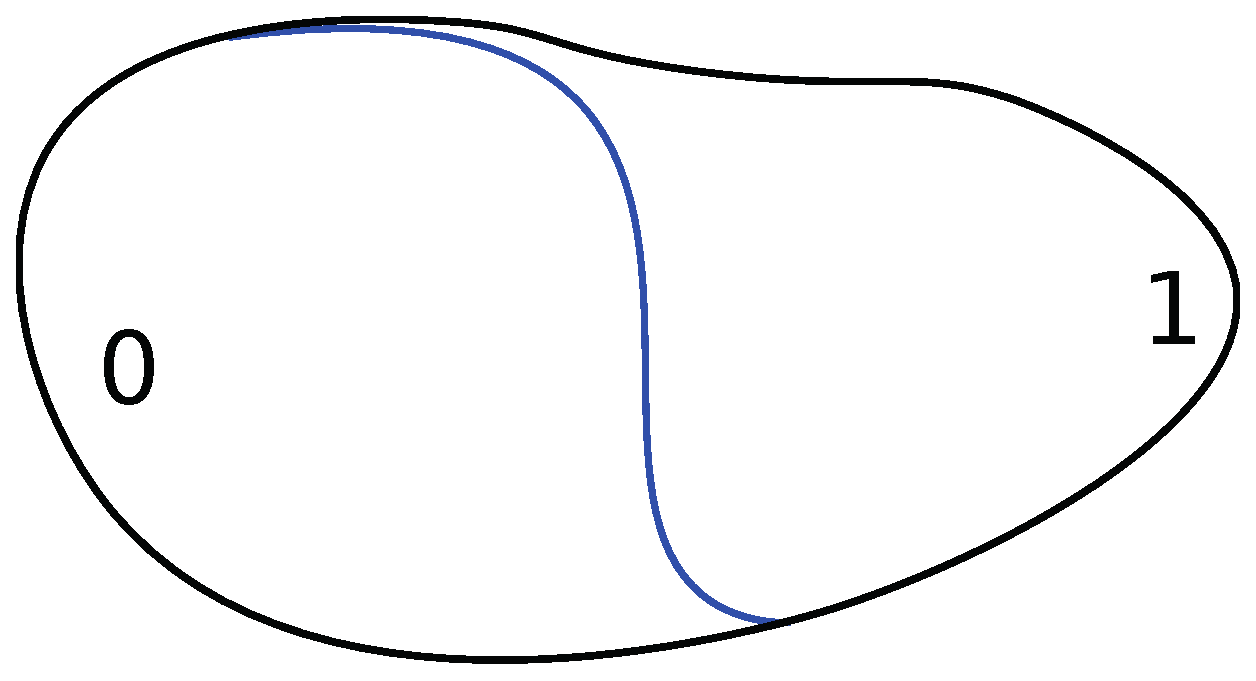
\includegraphics[width = 0.4\textwidth]{merge-opt2.eps}}\qquad \qquad
  \subfloat[Merge partitions ${\cal P}$\label{fig:merge-nhood}]{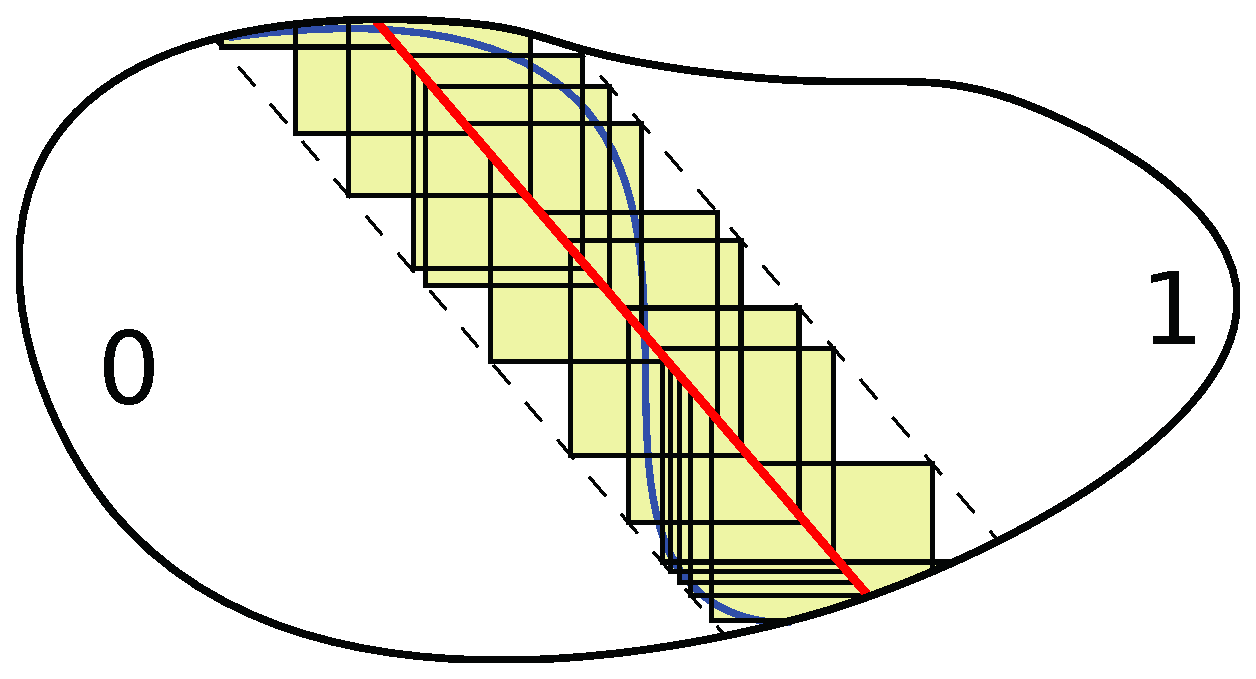
\includegraphics[width = 0.4\textwidth]{merge-nhood_red.eps}}\\[0.5cm] 
  \subfloat[Sub-problem solution $z^*$\label{fig:merge-sol}]{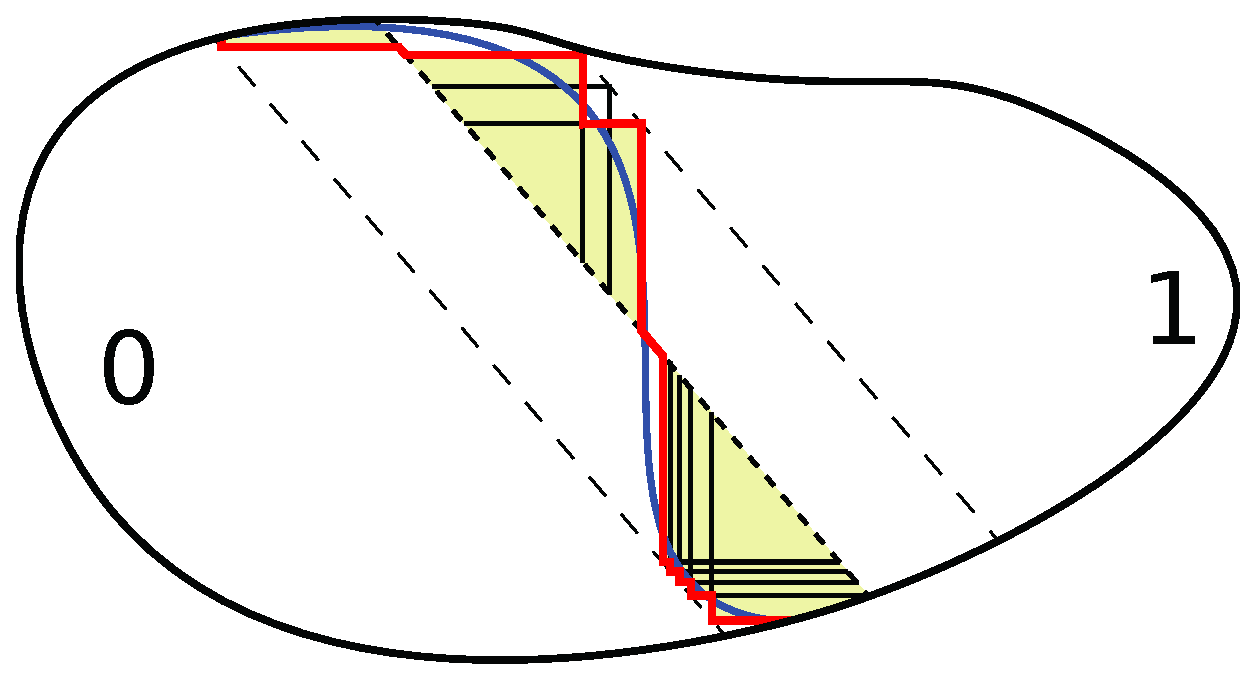
\includegraphics[width = 0.4\textwidth]{merge-sol.eps}}\qquad \quad
  \subfloat[Merged $f(x^k) \leq f(x^*)$\label{fig:merge-approx}]{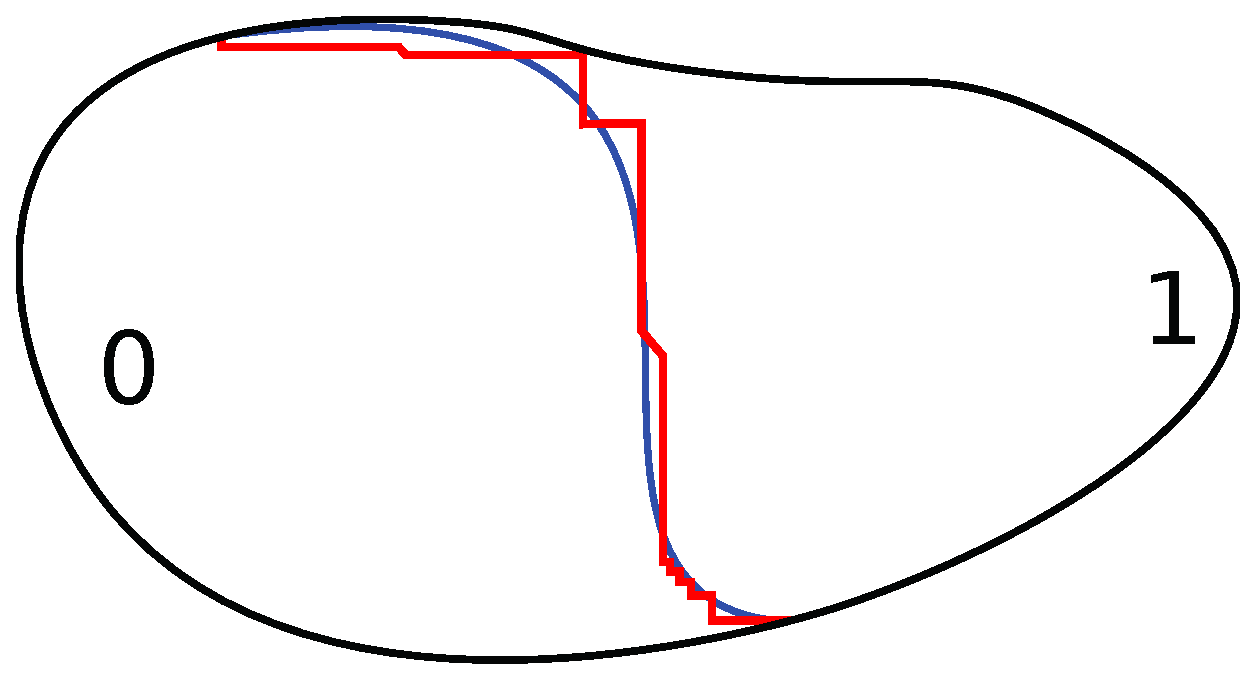
\includegraphics[width = 0.4\textwidth]{merge-approx.eps}}
  \caption{Solving the reduced sub-problem induced by the partitions ${\cal P}$, gives an approximate solution to the master problem.} 
    \label{fig:merge-solve}
\end{figure}

The partition on the decision variables representing the optimal solution $x^* \in {\cal F}$ is shown in blue in Figure~\ref{fig:merge-opt}. Figure~\ref{fig:merge-nhood} shows the merge partitions produced by merging the population $S$ and applying the random splitting heuristic. Here, the initial solution $x^{k-1}$ is the straight red partition boundary and each neighbouring solution in the population is represented by two triangular regions protruding from either side of this boundary. These regions represent the decision variables that take different values in the neighbouring solution, with respect to the initial --- regions on the left of the boundary indicate variables that have changed from 0 to 1 in the new solution, regions on the right indicate those that have changed from 1 to 0. The population is merged and split to produce the reduced sub-problem which is expressed in terms of a set of partition variables $z$. This reduced sub-problem is then solved using an exact solver or some other method. Figure~\ref{fig:merge-sol} shows that the optimal solution to the sub-problem $z^*$ is a partition constructed from a subset of the boundaries of the merge partitions. Finally, $z^*$ is mapped back to a solution to the master problem $x^k$ (Figure~\ref{fig:merge-sol}), an approximation of $x^*$. If the stopping criteria is not yet met, then the merged solution $x^k$ is used as the initial solution for the next iteration.

Provided there is at least one feasible solution in the population at the time of merging, the merged solution $x^k$ will always be feasible. As the merge partitions are formed by the intersections of all the members in the population $S$ (and then randomly split), any solution $s_i \in S$ can be reconstructed by simply including all partitions that are associated with that solution. This is illustrated in Figure~\ref{fig:group_part} above, where $s_1$ can be constructed by the union of partitions $P_2 \cup P_3 \cup P_5 \cup P_6$. If $s_i$ is feasible, then the final merge operation is able to produce $s_i$ as $x^k$; meaning that, so long as the initial solution $x^{k-1}$ is feasible, $x^{k-1}$ will be a lower bound on the solution produced by merging and $f(x^{k-1}) \leq f(x^k) \leq f(x^*)$, even if the entire rest of the population consists of randomly generated bit strings, representing infeasible solutions.


\subsection{Properties of Merge Search}
There are some simple but important properties that follow directly from the way this matheuristic has been defined.

\begin{lemma}\label{thm:improve}
  The Merge Step~\ref{step:merge} produces a solution that is at least as good
  as any of the neighbours in $S$: $f(x^k) \ge f(s)\ \forall s\in S$
\end{lemma}
\begin{proof}
  By construction any solution $s\in S$ satisfies $s\in \mathcal{F}$ and
  $s_i=s_j$ $\forall i,j\in P\in\mathcal{P}$ and so is feasible for the
  optimisation problem in Step~\ref{step:merge}. Hence, $f(x^k)\ge f(s)$.
\end{proof}

\begin{corollary}\label{thm:hill-climb}
  Merge Search is a hill-climbing method that produces a non-decreasing sequence
 of solution values: $f(x^0)\le f(x^1)\le f(x^2)\le \ldots$
\end{corollary}

Hence, for diversification, the method relies entirely on the neighbourhood
search in Step~\ref{step:nbhd} of the algorithm and the randomised splitting in
Step~\ref{step:RandSplit}. This is not a problem for large instances such as
this, where simply finding a very good local minimum is already a very
challenging task. Furthermore, the following property holds:

\begin{lemma}\label{thm:optimal}
  For pure binary problems where all variables are $0-1$, if random splitting of subsets is used in Step~\ref{step:RandSplit} (allowing any possible split with some non-zero probability) with $K\ge 2^{m+2}$ then Algorithm~\ref{alg:MS} is guaranteed to converge to the optimal solution as the number of iterations approaches infinity. 
\end{lemma}
\begin{proof}
  By assumption there exists an optimal solution in $\cal F$, due to the existence of $x^0\in\cal F$ and boundedness of $\cal F$ when all variables are binary. Let $s^*$ be any optimal solution. The first thing to note is that if a partition $\mathcal{P}^*$ satisfies $s^*_i=s^*_j\ \forall P\in \mathcal{P}^*,\ i,j\in P$ then the Merge problem in Step~\ref{step:merge} yields and optimal solution. 
  Such a partition could be generated, from any arbitrary partition $\cal P$ by splitting each $P\in\cal P$ into $P_0=P\cap \{i\mid s^*_i=0\}$ and $P_1=P\cap \{i\mid s^*_i=1\}$. This splitting at most doubles the number of elements in the partition. \\
  Now the same argument can be used to show that $|\mathcal{P}|$ as produced in Step~\ref{step:P} has at most $2^{m+1}$ elements (corresponding to splitting based on solutions $s^1,\ldots,s^m$ and $x^{k-1}$). Hence, we only need $K$ to be at least $2^{m+2}$ to allow some chance of generating the required partition in any step. Hence, as the number of iterations of Algorithm~\ref{alg:MS} goes to infinity the chance of \emph{not} producing an optimal solution goes to zero. And of course, based on Corollary~\ref{thm:hill-climb} once an optimal solution has been found, the algorithm will not depart from this.
\end{proof}
While convergence to the optimal solution is of course extremely unlikely for practical sized instances, the lemma shows that it is at least theoretically possible. Furthermore, while $2^{m+2}$ appears quite large, the only real requirement is that $K$ is sufficiently large to allow each element of $\cal P$ to be split once, with $|\mathcal{P}|$ typically much smaller than $2^{m+1}$ in practice. Hence, while Merge Search is a hill-climbing method, it is at least in principle possible for the method to reach a global optimum from any starting point.

\subsection{Comparison with CMSA}
As mentioned previously, it may be noted here that this meta-heuristic has some similarity to the recently published CMSA heuristic by \citet{cmsa}. Although there are some similarities between merge search and CMSA, there are two areas where merge search diverges significantly from it. These are:
\begin{itemize}
\item the generation of candidate solutions to be merged; and
\item the aggregation of decision variables in the reduced sub-problem.
\end{itemize}
The CMSA sub-problems are still defined based on a population of solutions, however these solutions are constructed probabilistically, with each solution being generated from scratch. This has the two-fold effect of reducing the capacity of CMSA to learn from the best individual solution found so far, and also makes it impractical when trying to solve large-scale, or very complicated, problems for which constructing a feasible solution is extremely time consuming, such as the CPIT problem that is considered here. Merge search avoids this issue by heuristically constructing an initial solution and then sampling its neighbourhood in order to generate a population, which is then used to define its sub-problems. The effect of this is to make the time taken to generate the population of solutions dependent on the local search algorithm used to sample the neighbourhood of a given feasible solution which is often much faster than the algorithm used to find feasible solutions from scratch. Of course, this leaves merge search potentially susceptible to being overly sensitive to the quality of the initial solution; however, this can be mitigated by increasing the diversity of the population, or further splitting the merge partitions. 

The second area where there is a significant divergence between the two methods is in the aggregation of decision variables. CMSA uses its population of constructed solutions to determine the variables that are to be included in its reduced sub-problem. If a variable is represented by an element of one of the candidate solutions in the population, it is automatically included in the reduced sub-problem. These variables are added to the sub-problem individually, and as such this aspect functions similarly to large neighbourhood search (LNS). One consequence of this is that the sub-problems can become very large, especially for problems where there are naturally many non-zero values in a solution. To combat this, a so-called ``ageing'' mechanism is introduced in CMSA to ensure that elements that have not been useful in producing good quality solutions recently are removed from the pool of solution elements. In contrast, merge search uses information from across the entire population to determine which variables are added into the reduced sub-problem as well as to aggregate variables that share common values across the population, and so likely share some kind of dependency. This grouping allows for more compact sub-problems and a much larger region of the search space can be covered for the same computational power. The trade-off for this is much coarser-grained solutions, however this can be alleviated by the introduction of random splitting to these groups to help escape local optima.

For a more thorough comparison between merge search and CMSA, see \citet{ms-vs-cmsa}.

\section{Merge Search in Practice}\label{sec:pract}
Section~\ref{sec:back} introduced the two problems that merge search was applied to in order to demonstrate its effectiveness and versatility: the constrained pit-limit (CPIT) problem; and the Steiner tree problem in graphs (STPG). This section gives the details of how merge search was applied to solve them.

\subsection{The CPIT problem}

\citet{gecco17} describe a novel representation for the precedence constrained production scheduling problem (PCPSP) --- a related problem to CPIT --- and a greedy randomised adaptive search procedure (GRASP) algorithm for solving it. They build on this with local search operator for the CPIT problem, and use it in a simple merge search framework that operates without variable partitioning or random splitting~\citep{gecco18}. By incorporating a variable partitioning mechanism, they show that a much larger region of the search space is able to be explored for the same computational budget~\citep{gecco19}. They exploit the structure of the problem, and treat many decision variables as a single group. This allows the size of the mixed-integer programming sub-problem to be greatly reduced and hence, the time required to solve it. A modified version of the CPIT formulation is given in Appendix~\ref{app:cpit} (Equation~\ref{eq:cpit_merge}).
\ak{put formulations in body}

The algorithm presented in this paper is an exentsion of this work, with two additions: a random splitting heuristic, to allow greater granularity in the solutions produced; and a ``solution polishing'' technique, based on the local improvement heuristic from the GRASP algorithm.

The random splitting heuristic is based on the local search neighbourhood in~\citep{gecco18}. An arbitrary variable in a partition is selected and all other variables that are in the predecessor cone for that variable, in the time-expanded problem graph, are computed and split from the partition. This preserves the precedence relationships between the relative position of blocks in time and space. As the number of variables in the reduced sub-problem increases with each split that is made, the size of the reduced sub-problem can be controlled; and this splitting process performed until the desired size is reached.

A solution polishing step is used to locally improve the best solution produced by merge search. A ``sliding window'' mechanism is employed which solves a reduced sub-problem that has all decision variables fixed except for those in time period $t$ and $t+1$, effectively allowing blocks to swap between time periods. The window of free variables is then moved to periods $t-1$ and $t$, and the process continues until the stopping conditions are met. This produces higher quality solutions, however the results in Section~\ref{sec:results} show that the combination of merge search and this polishing technique produces better results than by polishing alone.

\subsection{The Steiner tree problem in graphs}

% ---- REWRITE THIS PART

First described by \citet{kp:dowsland}, but subsequently used widely by many researchers, is the so-called key path neighbourhood. A key path is defined as a path within a Steiner tree where the two end vertices are either terminal vertices or vertices of degree at least 3; all intermediate  vertices (if any) are of degree 2 and are not terminal. The useful property of such structures is that their removal from a solution to the STPG will always result in two disconnected trees which can then be subsequently reconnected. This local search neighbourhood was extended by \citet{gecco16}, by adding a so-called ``jump'' operator which aids in escaping local minima, and is used as the basis of the merge search algorithm presented in this paper.

% ----
\begin{figure}[h]
\centering
\resizebox{0.9\linewidth}{!}{{}
    \includegraphics{stpg_merge.tikz}
    }
    \caption[Partitioning variables by merging solutions]{By merging two solutions (top left and right), the decision variables are partitioned into four disjoint sets, indicated here (bottom) by: red; blue; red and blue; and no colour.}\label{fig:stpg-partition} 
\end{figure}

The problem instance is first pre-processed using some of the techniques described in \citet{pp:duin,pp:uchoa,stpg-reduce} to reduce the number of decision variables. An initial solution is constructed and a neighbouring population produced, using the methods described in \citet{gecco16}. This population of solutions is used to partition the decision variables in the manner described in Section~\ref{sec:merge}, illustrated in Figure~\ref{fig:stpg-partition}.


These partitions can be split by selecting an arbitrary decision variable, and separating all variables representing vertices and edges that are connected to it and in the same partition. This ensures that any partition is split such that all variables removed from the original partition comprise a connected sub-graph, and as such should be able to be included in the resultant merged solution on its own, without the original partition. If a partition is split such that all variables are separated, leaving the original partition empty, then the last variable added to the split is kept in the original partition. As the connected variables are added using DFS, this is always a variable on the boundary, and so this method will not suffer from the problems present with truely random splitting. 

Having partitioned and split the decision variables, the resulting reduced sub-problem can be solved using a version of the \citet{goemans} MIP formulation that has been modified be expressed in terms of a single set of partition variables, instead of edge and vertex variables. The original Goemans \& Myung formulation and its merge search variation are included in Appendix~\ref{app:stpg} (Equations~\ref{eq:stpg_form} and~\ref{eq:stpg_merge}).
\ak{put formulations in body}

\section{Experiments}\label{sec:exper}
This section details the experimental set up, the experiments performed and finally presents the results and discusses the implications those results suggest.
\subsection{Datasets}
\subsubsection*{\textbf{The CPIT problem}}
Table~\ref{tab:datasets} details the properties of the problem instances used to test the algorithm in this paper. The instance name is given in the first column; followed by the number of blocks in the orebody model; the number of precedence arcs for each instance is provided in the third column; the fourth column gives the total number of time periods available; the number of decision variables is shown in the second last column; with the last column giving the total number of constraints in the problem model.\par
%
\begin{table}[h!]
\centering
\caption{Characteristics of \emph{minelib}~\citep{minelib} datasets.}\label{tab:datasets}
% \begin{adjustbox}{width=0.48\textwidth}
\begin{tabular}{lrrrrr} \toprule
Instance & Blocks & Precedences & Periods & Variables & Constraints\\
\hline
\texttt{newman1} & 1,060 & 3,922 & 6 & 6,360 & 29,904\\
\texttt{zuck\_small} & 9,400 & 145,640 & 20 & 188,000 & 3,100,840\\
\texttt{kd} & 14,153 & 219,778 & 12 & 169,836 & 2,807,196\\
\texttt{zuck\_medium} & 29,277 & 1,271,207 & 15 & 439,155 & 19,507,290\\
\texttt{marvin} & 53,271 & 650,631 & 20 & 1,065,420 & 14,078,080\\
\texttt{zuck\_large} & 96,821 & 1,053,105 & 30 & 2,904,630 & 34,497,840\\
\bottomrule
\end{tabular}
% \end{adjustbox}
\end{table}
%
A few instances from the full \emph{minelib} dataset were omitted due to missing files, referencing more than two resources or being too large for the algorithm in its current incarnation.

\subsubsection*{\textbf{The Steiner tree problem in graphs}}

The experiments were were carried out on categories $B$, $C$, $D$ and $E$ of the STPG problems from the \textit{steinlib} library~\citep{steinlib}, a standard dataset used by many researchers. The smaller-scale, category $B$ instances are 18 randomised networks with 50 to 100 vertices and 63 to 200 edges. The $C$ and $D$ datasets consists of 20 larger randomised networks, with 500 and 1,000 vertices, respectively, and between 625 to 25,000 edges. Finally, the $E$ dataset contains the largest instances, each with 2,500 vertices and between 3,125 and 62,500 edges. Details of the individual instances can be found in Table~\ref{tab:stpgprobs1} of Appendix~\ref{app:stein_data}. 

The optimal solutions for these instances are reported in the library and 
have been proven by exact methods such as branch-and-bound with graph reduction techniques.\par



\subsection{Pre-processing}
Being graph-based problems, both the CPIT problem and STPG are amenable to some amount of pre-processing. Detail about the pre-procesing methods used for the CPIT problem experiments can be found in \citet{gecco17}. For information about pre-processing techniques for the STPG, see \citet{pp:duin,pp:uchoa,stpg-reduce}.

\subsection{Experimental setup}
The experiments were carried out on an \emph{Intel{\textsuperscript{\textregistered}} Core{\textsuperscript{TM}} i5-2320} processor (3.0GHz) with 24GB RAM running Linux. All code was implemented in C++ with GCC-4.8.0. CPLEX Studio 12.7, operating with a single thread due to the need for callbacks, was employed as the mixed integer programming (MIP) solver. For the CPIT problem experiments, the boost library implementation of the Boykov-Kolmogorov algorithm was used to solve the UPIT sub-problem during the pre-processing stage.

\subsubsection*{\textbf{The CPIT problem}}
The merge search algorithm was compared against the baselines of the original results published on the \emph{minelib}~\citep{minelib} website, the most recent state-of-the-art results published in \citet{minelib-improved} and the results from using a greedy randomised adaptive search procedure (GRASP) heuristic, adapted from \citet{gecco17}. 

Also provided are the results for a variant of the merge search algorithm that uses variable grouping but no random splitting, previously published in \citet{gecco18}; and the results of combining merge search with a solution polishing phase. These are included in order to illustrate the effect that random splitting has on solution quality, and to demonstrate the effectiveness of combining an explorative technique with an exploitative one.Each algorithm was run 20 times on each instance, recording the mean objective value and standard deviation of the resulting solution produced by each run. 

\subsubsection*{\textbf{The Steiner tree problem in graphs}}
The merge search algorithm was compared against three separate baseline algorithms, the greedy randomised adaptive search (GRASP) heuristic, pure local search and pure MIP. The method of constructing initial solutions was different between the GRASP and merge search algorithms, so pure local search and pure MIP were included to ensure any improvement was not solely based on this factor. Aside from population merging, the merge search algorithm comprises two main components, local search and MIP search; so by isolating these two factors, it can be shown that merge search is greater than the sum of its parts.

Each algorithm was run 30 times on each (pre-processed) instance from the datasets, recording the mean objective value and standard deviation across all of the runs. All instances in the datasets used are supplied with their optimal objective values and this is used for the main stopping criteria. Otherwise, the stopping criteria of the merge search algorithm is generally dictated by the number of seconds spent in the MIP search so the time taken for each search is not provided, as it does not give much information about the performance of the algorithm. However, special mention is made when the algorithm terminated early for all runs.


Additional experiments were performed to investigate the difference between using the random and deterministic solution construction heuristics and the effect of population size on the size of the reduced sub-problem. In order to preserve space, a representative subset of the problem instances is used to illustrate the outcome of these experiments; however, these results are not ``cherry-picked'' and the full tables are available in Appendix~\ref{app:stpg_results}. 

\section{Results and discussion}\label{sec:results}
\subsection{The CPIT problem}

Table~\ref{tab:mine:main} provides the results of the three algorithms tested on the six problem instances from the \emph{minelib} dataset, along with the linear programming (LP) upper bound, the best solution as published on the \emph{minelib} website and the current best state-of-the-art solution as published in the survey paper from \citet{minelib-improved} --- ordered in ascending problem size.

\begin{table}[h]
\centering
\caption[Results on \emph{minelib} dataset instances]{Results on \emph{minelib} dataset instances. Given are the LP upper bound, the percentage gap between the LP bound and the best solution from the \emph{minelib} website; the best known solutions as published in \citet{minelib-improved} (with references to the original publications containing these results); the mean result from the GRASP heuristic; and the mean results from the merge search heuristic with no splitting, splitting and solution polishing, respectively.
}\label{tab:mine:main}
\begin{adjustbox}{width=\textwidth}
\begin{tabular}{lrrrrrrrrrr} \toprule
 & & & & & \multicolumn{3}{c}{merge search with:}\\
\cmidrule(lr){6-8}
Instance & \multicolumn{1}{c}{LP UB} & \multicolumn{1}{c}{\emph{minelib}} & \multicolumn{1}{c}{state-of-the-art}&\multicolumn{1}{c}{GRASP}&\multicolumn{1}{c}{no splitting} & \multicolumn{1}{c}{splitting}&\multicolumn{1}{c}{polishing}  \\ \midrule
%
\input mine/tables/gap_table_EJOR.tex
%
\bottomrule
\multicolumn{8}{l}{See: $^{[a]}$\citet{newman-improved}, $^{[b]}$\citet{zuck-small-improved}, $^{[c]}$\citet{aggregate}}
\end{tabular}
\end{adjustbox}
\end{table}

In this table, it can be seen that all three merge search variants consistently produce better results than the \emph{minelib} and the GRASP heuristic results, except for \newman{} and \zucklarge{}. The results for \newman{} are similar because the problem instance is so small and it can be assumed that the LP gap of 1.26\% is quite close to the optimal solution.

Comparing the results of the two variants of merge search (without polishing) illustrates the effect that random splitting has on the quality of the solution produced. For smaller problem instances, the two algorithms produce very similar quality solutions, indicating that the random splitting has little effect. However, as the size of the problem increases, the effect of the random splitting becomes more pronounced, with the biggest effect being on the two largest instances \zuckmed{} and \zucklarge{}\footnote{Although it is technically a larger problem than \zuckmed, solving the UPIT problem on the \marvin{} instance, as part of the pre-processing stage, eliminates many blocks and makes its effective size much smaller than \zuckmed.}. 

If there are no overlaps at all between variables across solutions, then the partitions in the reduced sub-problem are simply the set differences of the variables in each solution and the seed solution. In this extreme case, the merge operation is unable to produce a solution that does not already exist in the population, unless some random splitting of the partitions is performed. As the size of the problem instance decreases, the likelihood that there will be overlaps between variables across solutions increases. These overlaps in the variable sets produce splits in the partitions when producing the reduced sub-problem, reducing the need for additional random splitting to produce a different solution to those already existing in the generated population. This is not to suggest that random splitting would not be beneficial; but the problem with random splitting is that it is \emph{random}, and there is no way of guaranteeing that a particular split will improve the quality of a solution after merging, any more than a split produced by overlapping variable sets will.

The GRASP heuristic produces consistently worse results than merge search. This is expected as the sliding window heuristic used in the local improvement phase of the algorithm is better suited to incrementally improving a good solution than turning a mediocre solution into a good one, as it only operates on a small subset of the variables at one time. This means that it is good for ``tweaking'' a solution by shifting the time that a block is mined forward or backward one or two periods; but it is no good if the time that the block is mined must be moved by many periods, as this would take a lot of passes to achieve.

\subsubsection*{\textbf{Convergence behaviour}}

This idea of GRASP being better suited to incrementally improving an already good solution is demonstrated in Figure~\ref{plot:mine:runtime}. This figure gives the plots of the convergence behaviour of both the GRASP algorithm and merge search on all six of the CPIT instances. It can be seen in these plots that merge search converges quicker in nearly all instances, except for \dmine{}. 

\begin{figure}[!]
    \centering
    \begin{subfigure}[t]{0.3\textwidth}
    \centering
    \resizebox{\linewidth}{!}{
    \includegraphics{mine/plots/conv/newman1_conv.tikz}
    }
    \vspace*{-7mm}\caption{\newman{}}
    \label{plot:newman-conv}
    \end{subfigure}
    \quad
    \begin{subfigure}[t]{0.3\textwidth}
    \centering
    \resizebox{\linewidth}{!}{
    \includegraphics{mine/plots/conv/zuck_small_conv.tikz}
    }
    \vspace*{-7mm}\caption{\zucksmall{}}
    \label{plot:zuck-small-conv}
    \end{subfigure}
    \quad
    \begin{subfigure}[t]{0.3\textwidth}
    \centering
    \resizebox{\linewidth}{!}{
    \includegraphics{mine/plots/conv/kd_conv.tikz}
    }
    \vspace*{-7mm}\caption{\dmine{}}
    \label{plot:kd-conv}
    \end{subfigure}
    %
    \\[5mm]
    %
    \begin{subfigure}[t]{0.3\textwidth}
    \centering
    \resizebox{\linewidth}{!}{
    \includegraphics{mine/plots/conv/zuck_med_conv.tikz}
    }
    \vspace*{-7mm}\caption{\zuckmed{}}
    \label{plot:zuck-med-conv}
    \end{subfigure}
    \quad
    \begin{subfigure}[t]{0.3\textwidth}
    \centering
    \resizebox{\linewidth}{!}{
    \includegraphics{mine/plots/conv/marvin_conv.tikz}
    }
    \vspace*{-7mm}\caption{\marvin{}}
    \label{plot:marvin-conv}
    \end{subfigure}
    \quad
    \begin{subfigure}[t]{0.3\textwidth}
    \centering
    \resizebox{\linewidth}{!}{
    \includegraphics{mine/plots/conv/zuck_large_conv.tikz}
    }
    \vspace*{-7mm}\caption{\zucklarge{}}
    \label{plot:zuck-large-conv}
    \end{subfigure}
    \caption[Convergence plots for merge search on CPIT instances]{Convergence plots for CPIT instances. Merge search data is shown in blue and GRASP is shown in red. \ak{should i change these so that they are showing the LP gap instead of absolute value?}}
    \label{plot:mine:runtime}
\end{figure}

The difference here, is that the initial solution is already quite close in value to the resultant solution, so there are not a lot of improvements that can be made. This means that the more exhaustive search for small improvements of the GRASP algorithm is more likely to be effective, early on, than the more global search of the merge search algorithm, which relies on the stochastic natures of the local search operator and arbitrary splitting heuristic to find its improvements. Merge search does get there in the end --- and manages to find a slightly better solution in this case --- but it takes longer and with a more gentle curve. For all the other instances, where the gap between the initial and resultant solutions is much larger, merge search is demonstrably more suited to the task.

It can also be seen from these plots that once the algorithm has seemingly converged, it can sometimes find a way out of the local optima and locate a much better solution. This is evidenced in the plots for \zuckmed{}~(Figure ~\ref{plot:zuck-med-conv}), \marvin{}~(Figure~\ref{plot:marvin-conv}) and also Figure~\ref{plot:polish.med1} below. This behaviour is expected in such large problem instances, as once it has started to converge there are many ways to make the solution worse, but only a few to make it better; but once it has found a way out of the local optima, often several other improving moves will become apparent as well.

\subsubsection*{\textbf{Runtime information}}

Table~\ref{tab:mine:runtime} gives the runtime information (wall time and CPU time) for both GRASP and merge search. As they use a MIP solver to solve their restricted sub-problems, the runtime of both algorithms is reasonably easily configured by controlling how long the solver is allowed to run for each iteration. The parameters of the GRASP algorithm were chosen so that the search would take roughly the same amount of time as that of the merge search --- and for the most part, they are pretty similar. 

\begin{table}[h!]
\centering
\caption[Runtime information for experiments on CPIT]{Runtime information for experiments on CPIT. Given are the mean (\(\mu\)) and standard deviations (\(\sigma\)) of the wall and CPU time for the GRASP and merge search algorithms, in seconds.}\label{tab:mine:runtime}
\begin{adjustbox}{width=0.95\textwidth}
\begin{tabular}{lrrrrrrrr} \toprule
 & \multicolumn{4}{c}{GRASP} & \multicolumn{4}{c}{merge search}\\
\cmidrule(lr){2-5} \cmidrule(lr){6-9}
 & \multicolumn{2}{c}{Wall time [s]} & \multicolumn{2}{c}{CPU time [s]} & \multicolumn{2}{c}{Wall time [s]} & \multicolumn{2}{c}{CPU time [s]}\\
\cmidrule(lr){2-3}\cmidrule(lr){4-5} \cmidrule(lr){6-7}\cmidrule(lr){8-9}
Instance & \multicolumn{1}{c}{\(\mu\)}&\multicolumn{1}{c}{\(\sigma\)} & \multicolumn{1}{c}{\(\mu\)}& \multicolumn{1}{c}{\(\sigma\)}& \multicolumn{1}{c}{\(\mu\)}&\multicolumn{1}{c}{\(\sigma\)} & \multicolumn{1}{c}{\(\mu\)}& \multicolumn{1}{c}{\(\sigma\)}\\ \midrule

\input mine/tables/runtime_table.tex

\bottomrule
\multicolumn{9}{l}{\(^*\)population size for \zucklarge{} set at 500 for merge search due to insufficient memory.}
\end{tabular}
\end{adjustbox}
\end{table}
%

The two instances that are significantly different in runtime between GRASP and merge search are \dmine{} and \zucklarge{}. The reason that \zucklarge{} is so different is that it was impossible to run the merge search algorithm with a population of 1,000 on such a large problem instance, due to memory issues (even with 23 GB of RAM!); so a smaller population size of 500 was used, which took much less time to produce and to compute the merge partitions.

The reason for the differences in runtime on \dmine{} is illustrated in Figure~\ref{plot:mine:time}.
This figure shows plots of the amount of wall time in seconds consumed per iteration of the respective algorithms. The GRASP algorithm is measured by ``window movements'', which counts the number of times the window has incremented forwards or backwards along the solution. The merge search algorithm is measured by iterations; each the time for each iteration is measured at the point when a new candidate solution is generated for the population, so it is clear to see that, with a population size of one thousand, every thousandth iteration will include an extra amount of time to include the merge operation itself. 

\begin{figure}[h!]
    \centering
    \begin{subfigure}[t]{0.45\textwidth}
    \centering
    \resizebox{\linewidth}{!}{
    \includegraphics{mine/plots/time/zuck_small_grasp_time.tikz}
    }
    \caption{}
    \label{plot:time.1}
    \end{subfigure}
    \qquad
    \begin{subfigure}[t]{0.45\textwidth}
    \centering
    \resizebox{\linewidth}{!}{
    \includegraphics{mine/plots/time/zuck_small_merge_time.tikz}
    }
    \caption{}
    \label{plot:time.2}
    \end{subfigure}
    \caption[Plot of wall time {[s]} for \zucksmall{} and \dmine{} instances]{Plot of wall time [s] for \zucksmall{} (red) and \dmine{} (blue) instances. Sub-figure (\subref{plot:time.1})~shows GRASP algorithm data and (\subref{plot:time.2})~shows merge search data.}
    \label{plot:mine:time}
\end{figure}
%

It is important to remember here that the \dmine{} instance only has a maximum of 12 periods allowed, while \zucksmall{} has 20. So, while the number operations for GRASP is dependent on the number of periods (and therefore window movements), merge search is dependent on population size. This is demonstrated very clearly in Figure~\ref{plot:time.2}, where there is very little difference between the two instances. It can be seen that the population is generated reasonably quickly (indicated by the flat parts of the curve) and then each point where there is a sudden jump in the amount of time taken indicates that a merge operation has taken place.


But this is not the end of the story. In these two examples, GRASP took 2,979 seconds to complete the search on \dmine{} and it took 4,180 to complete the search on \zucksmall{}. If there was a direct linear relationship between time taken to complete the search and number of periods, the amount of time GRASP should take to complete its search on \zucksmall{} should be \(\frac{2,979\times20}{12} = 4,965\). So where did the other 13 minutes go?

Looking at Figure~\ref{plot:time.1}, the main thing that can be noticed here is that the shape of the plot for \zucksmall{} is significantly different to the shape of the plot for \dmine{}. The regular flat spots in the plot for \zucksmall{} indicate that there is a group of periods for that problem that are not used by the solution, or do not contain any blocks that can be moved around, and therefore the MIP solver will not take the full amount of allowed time to solve the reduced sub-problem. It so happens that the solution to \zucksmall{} does not use any period after period 16, so the first and last few window moves of each full pass take very little time at all. In contrast the \dmine{} instance uses periods right up until period 10, so there are fewer window moves that will be skipped over, as evidenced by the straighter line on the plot.


\subsubsection*{\textbf{Solution polishing}}
 
The results in the last column of Table~\ref{tab:mine:main} show the effect of combining merge search with the local improvement heuristic from the GRASP algorithm. These results clearly demonstrate the effectiveness of this combination, even improving the best known bounds for \dmine{} and \zucklarge{}. 

For these experiments, the best solution from the merge search runs is taken and then three passes of the sliding window heuristic is applied. Although doing this effectively increases the allowed computational budget, the quality of the solutions produced by doing this is better than if the computational budget is increased for either of the two algorithms on their own. In the case of the GRASP algorithm, the quality of the solution at the end of its run is still too low to be able to improve the objective value by very much in only three passes. In the case of the merge search algorithm, because both the population generation and merge partition splitting occurs stochastically, as the quality of the solution increases the chances of finding an improving solution, or partition split, by chance decreases. This means that the search is likely to have converged by the end of its run, so increasing the computational budget at this point is unlikely to produce much of an improvement in the quality of the solution, if any at all.

Applying the sliding window heuristic at the end of the merge search process solves both of these problems. The sliding window heuristic performs a much more methodical and exhaustive search to find small improvements that can be made to the solution which might be difficult to find by random sampling, in such a large search space. Additionally, by starting the sliding window heuristic with a much higher quality initial solution, computational effort does not need to be wasted on the ``low hanging fruit'' that can be found easily by sampling the search space. As the heuristic only considers a small subset of the variables at a time, it cannot make large changes to the solution in a single iteration. 

Figure~\ref{plot:mine:polish} contains plots that illustrate this concept on two instances of the CPIT problem, \zuckmed{} and \zucklarge{}. The left-hand sub-figures show the full process with both merge phase (shown in blue) and polishing phase (shown in red). Figure~\ref{plot:polish.med1} demonstrates the power of intensification of the search with the sliding window heuristic. Here, the blue merge plot can seen to have effectively converged as there has been no significant improvement in objective value for over half an hour of wall time. Applying the sliding window heuristic to this ``converged'' solution results in an almost immediate improvement, followed by subsequent improvements, before this too converges to its local optimum.


\begin{figure}[h]
    \centering
    \begin{subfigure}[t]{0.4\textwidth}
    \centering
    \resizebox{\linewidth}{!}{
    \includegraphics{mine/plots/polish/zuck_med_polish.tikz}
    }
    \vspace*{-5mm}\caption{\zuckmed{}}
    \label{plot:polish.med1}
    \end{subfigure}
    \qquad \qquad
    \begin{subfigure}[t]{0.4\textwidth}
    \centering
    \resizebox{\linewidth}{!}{
    \includegraphics{mine/plots/polish/zuck_med_grasp_polish.tikz}
    }
    \caption{Detail of polishing phase}
    \label{plot:polish.med2}
    \end{subfigure}
    %
    \\[0.5cm]
    %
    \centering
    \begin{subfigure}[t]{0.4\textwidth}
    \centering
    \resizebox{\linewidth}{!}{
    \includegraphics{mine/plots/polish/zuck_large_polish.tikz}
    }
    \vspace*{-5mm}\caption{\zucklarge{}}
    \label{plot:polish.large1}
    \end{subfigure}
    \qquad \qquad
    \begin{subfigure}[t]{0.4\textwidth}
    \centering
    \resizebox{\linewidth}{!}{
    \includegraphics{mine/plots/polish/zuck_large_grasp_polish.tikz}
    }
    \vspace*{-5mm}\caption{Detail of polishing phase}
    \label{plot:polish.large2}
    \end{subfigure}
    \caption[Plot of merge search with solution polishing on \zuckmed{} and \zucklarge{} instances]{Plot of merge search with solution polishing on \zuckmed{} and \zucklarge{} instances. Figures (\subref{plot:polish.med1}) and (\subref{plot:polish.large1}) show the merge search (blue) and polishing (red) phases; Figures (\subref{plot:polish.med2}) and (\subref{plot:polish.large2}) show details of the polishing phases.}
    \label{plot:mine:polish}
\end{figure}

Not as emphatic in demonstrating this point are the results presented in Figure~\ref{plot:polish.large1}. It can be seen in this figure that merge search was still a ways off from converging, although it had started to slow its progress. It could be argued that, were merge search allowed to continue, it would have found the same solution eventually. Although, it can be seen in the plot that applying the polishing heuristic to this unconverged solution did still result in an initial rapid increase in solution quality; and as merge search was beginning to tail off, it probably would have taken longer to reach its goal.

The results from these experiments suggest that, while merge search is adept at finding a good quality global solution, it benefits from the addition of a more exhaustive local method to intensify its search. 


\subsection{The Steiner tree problem in graphs}

Table~\ref{tab:stpg:results:trunc} provides a representative sample of the results for the experiments performed to compare the merge search algorithm to the three base-line algorithms of GRASP, pure local search and pure MIP. Given is the known optimal solution, and the percentage gap between the optimal and the mean objective value from all of the runs. The best results for each problem instance are indicated in bold; and, as the optimal solution is known for each instance, if the algorithm managed to find the optimal solution in any of its runs, this is indicated by an asterisk --- clearly, if a result has a gap of 0.00\%, this indicates the optimal solution was found in every run. The full results are available in Appendix~\ref{app:stpg_results}.


The results for the \(B\) dataset show that merge search demonstrably outperformed all of the algorithms it was tested against, as do the rest of the datasets. In this first dataset comprised of all the smallest sized instances (around 60 to 290 decision variables, pre-processed), merge search performed the best; managing to find the optimal solution in every run for every problem instance, with many terminating in the first couple of iterations. The next most successful algorithm was the pure MIP algorithm\footnote{It should be pointed out here that the pure MIP algorithm failed to produce even a single integer solution for most of the problem instances in the time allotted to it, if it was not given a heuristically constructed solution as a warm start. Therefore the success of the pure MIP algorithm over the GRASP algorithm for this dataset should be attributed to the fact that the MIP search was initially seeded with a higher quality solution than the GRASP algorithm.}, which just edges out pure local search and finally followed by GRASP at the end. The fact that both pure local search and pure MIP outperformed GRASP suggests that the quality of the initial solution is very important to the quality of the resultant solution --- especially in these smaller problem instances --- so, as pure local search and pure MIP both use the same, deterministic, solution construction as merge search, they are likely to perform better than GRASP, which uses the random solution construction heuristic.

\begin{table}[h!]
\centering
\caption{Representative sample of results across \emph{steinlib} dataset instances, giving the optimality gap for the mean objective value of pure local search, pure MIP, GRASP and merge search, respectively. An asterisk indicates that the optimal solution was found at least once in all the runs.}\label{tab:stpg:results:trunc} 
% \begin{adjustbox}{width=0.45\textwidth}
\begin{tabular}{lrrrrr} \toprule
Instance & Opt. & pure LS & pure MIP & GRASP & merge search\\ \midrule
%
\input stpg/tables/trunc_gap.tex
%
\bottomrule
\end{tabular}
% \end{adjustbox}
\end{table}

The picture begins to change slightly with the results for the \(C\) dataset. Merge search is still the clear winner of the four here; although it has not managed to achieve the optimal solution in every single one of its runs and has actually failed to reach the optimal solution in a few of the instances. The big change here is the fact that pure MIP has fallen to last place for almost every single problem instance, even with the warm start seeding; and by the \(D\) dataset it is last in every problem instance. This suggests that, by the time the problem instances reach even this moderate size (between 400 and 5,280 decision variables), the problem is too large to be solved by a MIP solver alone, using comparable computing resources. This is evidenced by the fact that the standard deviation is zero (see Appendix~\ref{app:stpg_results}) for many of the instances, suggesting that it had a hard time finding a better solution than it was seeded with. 

It is worth mentioning that some of the state-of-the-art results in the \emph{steinlib} library have been produced by a combination of pre-processing and integral LP formulation, so this does not mean that these results suggest the problems are too large for MIP solvers in general, merely that they are too large for the simple formulation used for this research. Better, more complicated MIP formulations for the STPG are available~\citep{goemans,stpg-improved,hypergraph}; however, these experiments are not intended to advance the state-of-the-art for STPG solvers, but to demonstrate the application of merge search to the STPG and that there is a non-trivial benefit that can be gained from doing so. If both pure MIP and merge search used better formulations, and more sophisticated pre-processing techniques, they would indeed be able to achieve better quality solutions; but one could expect a similar gulf in quality between the pure MIP and merge search to emerge --- albeit, on much larger problem instances.

The trend of pure local search outperforming the GRASP heuristic continues throughout the rest of the datasets, with the exception of problem instances \texttt{c11}, \texttt{d06}, \texttt{d16} and \texttt{e02}. Differences between the mean objective values for these instances are small enough to suggest that these are anomalous and probably the result of the random construction heuristic finding a better initial solution to the deterministic heuristic, or simple luck during the local search. 

The fact that pure local search outperformed GRASP in nearly every problem instance suggests that the choice of initial solution is very important to the quality of the solution produced, as otherwise, these two algorithms are nearly identical; so the use of the deterministic construction heuristic is preferable to the random one. Added to this, the fact that merge search equals --- or outperforms --- pure local search in every problem instance suggests that there is indeed a benefit to creating a hybrid meta-heuristic using a MIP solver that solves a reduced sub-problem induced by merging a population of solutions produced by the local search neighbourhood. Finally, the fact that the merge search algorithm equals --- or outperforms --- the pure MIP algorithm in every problem instance suggests that these benefits that are gained are not simply from the addition of a MIP solver itself; and therefore, must be the result of the hybridisation and population merging processes.

\subsubsection*{\textbf{Additional experiments}}

The results in Table~\ref{tab:stpg:pop:trunc} show the effect that changing the population size has on the number of partitions in the resultant reduced sub-problem, before random splitting is applied. It can be seen from the data that as the size of the population increases, the number of partitions also increases. This is to be expected, as two variables are included in the same partition only if they agree on values across the entire population of solutions; therefore, if more solutions are considered, the less likely variables are to agree across them all and the more partitions in the reduced sub-problem. Again, these are just a representative set of the problem instances, the full results are given in Table~\ref{tab:app:pop} of the appendix.

\begin{table}[h!]
\centering
\caption[Size of reduced sub-problem results]{Representative sample of results across \emph{steinlib} dataset instances, investigating the effect that population size has on the number of partitions in the reduced sub-problem. Given are the size of the instance (\(|V|+|E|\)) and average number of partitions and standard deviation over 30 runs for population sizes 50, 100, 1,500 and 10,000.}\label{tab:stpg:pop:trunc} 
\begin{adjustbox}{width=0.9\textwidth}
\begin{tabular}{lrrrrrrrrr} \toprule
 &  & \multicolumn{2}{c}{50} & \multicolumn{2}{c}{100} & \multicolumn{2}{c}{1,500} & \multicolumn{2}{c}{10,000}\\
\cmidrule(lr){3-4} \cmidrule(lr){5-6} \cmidrule(lr){7-8} \cmidrule(lr){9-10} 
Instance & size & \multicolumn{1}{c}{\(\mu\)}&\multicolumn{1}{c}{\(\sigma\)} & \multicolumn{1}{c}{\(\mu\)}&\multicolumn{1}{c}{\(\sigma\)}& \multicolumn{1}{c}{\(\mu\)}&\multicolumn{1}{c}{\(\sigma\)} & \multicolumn{1}{c}{\(\mu\)}&\multicolumn{1}{c}{\(\sigma\)}\\ \midrule
%
\input stpg/tables/trunc_pop.tex
%
\bottomrule
\end{tabular}
\end{adjustbox}
\end{table}

Figure~\ref{fig:stpg_pop_plots} shows some of the plots that were used in the sensitivity analysis done to determine an appropriate population size for these experiments. The number of partitions in the reduced sub-problem was plotted against population size from 0 to 5,000 and a population size of 1,500 was decided upon for two main reasons. The first reason is that it can be seen in the plots that although the number of partitions is proportional to the population size, it is not directly proportional, and after a certain inflection point there are significant diminishing returns in the number of partitions for population size. It can be seen from the plots that the position of this inflection point moves further to the right with the size of the problem and it was decided that 1,500 was a decent value that could be used across the whole dataset. It is slightly after the inflection point for most of the \(C\) dataset instances and slightly before the inflection point for most of the \(D\) dataset instances. The \(B\) dataset instances are small enough that it doesnt matter that 1,500 is probably too many and, although it falls very short of the \(E\) dataset instances inflection point, larger population sizes produce too many partitions for the MIP solver to handle.
%
\begin{center}
\begin{figure}[h]
    \centering
    \begin{subfigure}{0.4\textwidth}
    \centering
    \resizebox{\linewidth}{!}{
    \includegraphics{stpg/plots/b10_pop_plot.tikz}
    }
    \caption{Instance \texttt{b10}}
    \label{fig:stpg_pop.1}
    \end{subfigure}
    \qquad \qquad
    \begin{subfigure}{0.4\textwidth}
    \centering
    \resizebox{\linewidth}{!}{
    \includegraphics{stpg/plots/c10_pop_plot.tikz}
    }
    \caption{Instance \texttt{c10}}
    \label{fig:stpg_pop.2}
    \end{subfigure}
    \\[0.5cm]
    \begin{subfigure}{0.4\textwidth}
    \centering
    \resizebox{\linewidth}{!}{
    \includegraphics{stpg/plots/d10_pop_plot.tikz}
    }
    \caption{Instance \texttt{d10}}
    \label{fig:stpg_pop.3}
    \end{subfigure}
    \qquad \qquad 
    \begin{subfigure}{0.4\textwidth}
    \centering
    \resizebox{\linewidth}{!}{
    \includegraphics{stpg/plots/e10_pop_plot.tikz}
    }
    \caption{Instance \texttt{e10}}
    \label{fig:stpg_pop.4}
    \end{subfigure}
    \caption[Effect of population size on number of partitions in the reduced sub-problem]{Effect of population size on number of partitions in the reduced sub-problem. Dotted line shows population size of 1,500, which was used for these experiments.} 
    \label{fig:stpg_pop_plots}
\end{figure}
\end{center}
%
The second reason for choosing this population size is that in order for the MIP solver to be effective, the number of decision variables must be kept at a reasonable amount. It was decided that the number of partitions in the reduced sub-problem, after random splitting, should a maximum of around 2,000, on average. The number of random splits was set at 500, therefore the number of partitions before splitting should be around a maximum of 1,500 --- which occurs at a population size of around 1,500 for many of the problem instances. For larger problem instances which need a larger reduced sub-problem, an extra parameter was added, which ensures that the reduced sub-problem is some fraction of the total instance size.

\section{Conclusion and future work}

Constrained optimisation problems involve the search for an optimal object in (often \emph{very} large) search spaces --- in the case of combinatorial optimisation, these spaces are finite and discrete. As well as this, problems that are abstractions of real-world processes can be extremely complex; having many additional side-constraints, separate to the main problem constraints themselves, which must be considered when modelling the problem mathematically.

\citet{np:karp} showed that NP-Complete problems are all theoretically reducible to one another; however, in practice, they often require specific domain knowledge that requires the development of custom algorithms for each case. The discovery of a ``one size fits all'' solution for this class of problems would be a vital achievement in the field of operations research, and the purpose of this research is to attempt to provide a material step in the direction towards this goal.

Merge search, the algorithm proposed here, is a generalised hybrid meta-heuristic framework for solving large-scale and complex constrained optimisation problems --- with, or without specific domain knowledge. The operation of this framework can be broken down into several phases:
\begin{itemize}
\item \emph{Initial solution construction:} a feasible solution to the problem is constructed, either heuristically or by solving a generic mixed integer program (MIP) model of the problem that penalises non-feasible solutions;
\item \emph{Population generation:} a population of neighbouring solutions is generated, using some local search heuristic or by randomly perturbing an initial solution;
\item \emph{Partitioning variables:} the population of solutions is used to determine how the set of decision variables are partitioned. Additional splits to these partitions can be made to increase the granularity of the solutions produced; and,
\item \emph{Solving reduced sub-problem:} new local optima can be found by solving a reduced version of the problem which uses each partition as a meta-variable, either with a MIP solver or by some other method. By grouping the decision variables, this sub-problem requires much less computational effort to solve --- the trade-off being that the solution produced becomes an approximation of the optimal one.
\end{itemize}

A theoretical description of merge search was given and it was also shown that merge search can be considered a generalisation of many optimisation techniques such as crossover and mutation operators in genetic algorithms, or search techniques like large neighbourhood search.

Practically, two problems were used as testing-grounds to demonstrate the effectiveness of merge search and explore some of its features and facets. The first was a complex, real-world problem from the field of open-pit mining called the constrained pit-limit (CPIT) problem and the second was a well-known problem from Karp's original 21 NP-Complete problems, the Steiner tree problem in graphs (STPG). These two problems were chosen because they are very dissimilar and require very different approaches to solve them, which allowed the versatility and flexibility of this hybrid meta-heuristic framework to be showcased.

As it is a much simpler problem, the experiments on the STPG were used to investigate some of the main properties and design choices of merge search. In contrast, the experiments on the CPIT problem highlighted the effectiveness of merge search in solving large scale, highly constrained, problems through its automatic decomposition aspects. They also investigated the effect that additional arbitrary splitting of the merge partitions has on the quality of the solutions produced and also the inclusion of a solution polishing phase afterwards.

While the datasets used for the STPG experiments already had been solved to optimality, and therefore were only being used to demonstrate the versatility of merge search and investigate its various aspects; the experiments on the CPIT problem produced solutions which improved on the upper-bounds of all six of the problem instances, as published on the \emph{minelib} website, and two of the most recent published upper-bounds as reported in \citet{minelib-improved}.

\smallskip

Although demonstrating that merge search can be applied to two very different problems shows that the algorithm is very versatile, making the claim that it is a general framework that can be applied to \emph{any} combinatorial optimisation problem would require significantly more evidence than only two problems. Therefore, the most obvious future research that can be performed is in applying the technique to many more (and varying types of) problems. Aside from this, some further work could be done into developing a truly generic algorithm which operates entirely on the decision variables, and is completely problem agnostic; the interaction of different heuristics and other techniques, within the framework; the effectiveness of merge search with other exact solvers (such as constraint programming); the limits at which merge search is most effective; and, applying merge search to different classes (possibly non-discrete) of problems.

\section*{References}

\bibliography{merge_refs.bib}

\appendix
\section{CPIT Formulations}\label{app:cpit}
\subsection*{Espinoza formulation}
Espinoza et al. describe a mathematical programming formulation for the CPIT problem~\citet{minelib} which maximises the discounted profit summed over all blocks $b \in \S{B}$ and time periods $t \in \S{T}$, multiplied by the value of the decision variables $x_{bt}$. In their formulation, the variable $x_{bt}$ is equal to 1 if block $b$ is excavated at time $t$ and 0 otherwise.\par 

The data for the CPIT problem consists of the following sets and parameters:

% {\renewcommand{\arraystretch}{1.2}% for the vertical padding
\begin{tabular}{p{0.05\linewidth}p{0.85\linewidth}}
$\S{B}$ & the set of blocks;\\
$\S{T}$ & the set of time periods;\\
$\S{R}$ & the set of resources. Typically, $|\S{R}| = 2$;\\
$\mathcal{P}$ & the set of precedences. $a \to b$ if $(a,b) \in \mathcal{P}$
                means block $a$ must be mined before block $b$;\\
$\hat{p}_{bt}$  & the discounted profit for mining block $b$ at time $t$
            (can be negative if it is a cost only). This
            is simply $\frac{p_b}{(1+\alpha)^t}$ for some base cost
            $p_b$ and a discount value typically 0.1;\\
$q_{br}$ & the amount of resources required to extract block $b$;\\
$\overline{\S{R}}_{rt}$ & the maximum amount of resource $r$ available in time period $t$; and\\\hfill\\
$\underline{\S{R}}_{rt}$ & the minimum amount of resource $r$ that must be consumed in time period $t$ (typically 0).\\\hfill\\
\end{tabular}
% }
\par
The variables used to solve this problem are:\\\hfill\\
\begin{tabular}{p{0.05\linewidth}p{0.85\linewidth}}
$x_{bt}$ & is a matrix of binary variables in $\Bin^{|\S{B}||\S{T}|}$ that are 1 if block $b$ is mined in
                      period $t$ and 0 otherwise.\\\hfill\\
\end{tabular}

Using this notation, the problem is written as:

{\footnotesize
\begin{align}
\Max \quad & \displaystyle\sum_{b \in \S{B}}\displaystyle\sum_{t \in \S{T}} \hat{p}_{bt}x_{bt},\label{eq:cpit_form}\\
\ST \quad & \displaystyle\sum_{\tau \leq t}x_{b\tau} \leq \displaystyle\sum_{\tau \leq t}x_{a\tau} \qquad \qquad & \forall\ (a,b) \in \mathcal{P}, t \in \S{T},\nonumber\\
& \displaystyle\sum_{t \in \S{T}}x_{bt} \leq 1 & \forall\ b \in \S{B},\nonumber\\
& \underline{\S{R}}_{rt} \leq \displaystyle\sum_{b \in \S{B}}q_{br}x_{bt} \leq \overline{\S{R}}_{rt} & \forall\ r \in \S{R}, t \in \S{T},\nonumber\\
& x_{bt} \in \Bin & \forall\ b \in \S{B}, t \in \S{T}\nonumber.
\end{align}
}

\subsection*{Merge search formulation}

By aggregating the block-time decision variables into groups, the problem can be reduced significantly by modifying the Espinoza formulation given above such that each group $G_i \in \S{G}^p$ is represented by a new variable $z_i$: 
{\footnotesize
\begin{align}
\Max \qquad & \displaystyle\sum_{G_i \in \S{G}^p} p_{i}z_i,\label{eq:cpit_merge}\\
\ST \qquad & z_j \leq z_i \qquad \qquad & \forall\ (i,j) \in \mathcal{P}^G, \nonumber\\
& \displaystyle\sum_{G_i \in \S{G}^p}q_{ir}z_i \leq \displaystyle\sum_{t \in \S{T}}\overline{R}_{r} & \forall\ r \in \S{R}, \nonumber\\
% & \displaystyle\sum_{b \in B}q_{b}(x_{bt} - x_{bt-1}) \leq \overline{R}_{t} & \forall\ t \in T,\label{res-t}\\
& z_i \in \Bin & \forall\ G_i \in \S{G}^p \nonumber.
\end{align}
}
Here, the objective value now becomes the sum of the cumulative profits for all groups that are included in a solution. Because the $x_{bt}$ variables were cumulative, but the $z_i$ variables are not, computing the total value of a given group or its resource usage becomes a bit complicated.

\begin{definition}
Let $G_i \in \S{G}^p$ be a group of cumulative \(x_{bt}\) binary decision variables where \(x_{bt} = 1\) means that block $b$ is extracted at time $t$ or earlier. Then, \(\alpha_{bi} = \min\{t \mid x_{bt} \in G_i \land x_{bt} = 1\}\) is the earliest time that block \(b\) appears in group \(G_i\) and \(\omega_{bi} = \min\{t \mid x_{bt} \in G_i \land x_{bt} = 1\}\) is the latest.
\end{definition}

\begin{prop}\label{prop:merge-group-profit}
The total value that $G_i$ contributes to the NPV of the mine is given by: $p_i = \sum_{b \in \S{B}} \hat{p}_{b\alpha_{bi}} - \hat{p}_{b\omega_{bi}+1}$. If $\omega_{bi} = |\S{T}|$ then $\hat{p}_{b\omega_{bi}+1} = 0$ and if \(\alpha_{bi} = \emptyset\) then \(\hat{p}_{b\alpha_{bi}} - \hat{p}_{b\omega_{bi}+1} = 0\).
\end{prop}
%
Because the $z_i$ variables are not cumulative, the time-precedence constraints can be merged with the space-precedence ones. 
\begin{prop}\label{prop:merge-group-prec}
The set of group precedences $\mathcal{P}^G \subseteq \S{G}^p \times \S{G}^p$ is: $\{(G_i,G_j) \mid (a,b) \in \mathcal{P}, x_{at} \in G_i, x_{bt} \in G_j, \forall t \in \S{T}\} \cup \{(G_i,G_j) \mid x_{bt} \in G_i, x_{bt+1} \in G_j, \forall b \in \S{B}\}$.
\end{prop}

The cumulative resource usage for a given group $G_i$ can be computed in much the same way as the cumulative profit. This differs to the Espinoza formulation in that the sum of the cumulative resource usage must be less than or equal to the total resource limit over the entire life of the mine, not per period.
\begin{prop}\label{prop:merge-group-resource}
The total amount that $G_i$ contributes to the resource consumption is: $q_{ir} = \sum_{b \in \S{B}} q_{br}x_{b\alpha_{bi}} - q_{br}x_{b\omega_{bi}+1},\ \forall r \in \S{R}$. If $\omega_{bi} = |\S{T}|$ then $q_{br}x_{b\omega_{bi}+1} = 0$ and if \(\alpha_{bi} = \emptyset\) then \(q_{br}x_{b\alpha_{bi}} - q_{br}x_{b\omega_{bi}+1} = 0\).
\end{prop}
%
Having constructed this reduced sub-problem in terms of the new $z_i$ group variables, it can be solved using a MIP solver and the solution is then used as the seed solution for a new population.

% you can choose not to have a title for an appendix
% if you want by leaving the argument blank
\section{STPG Formulations}\label{app:stpg}
\subsection*{Goemans and Myung formulation}
The following formulation is from Goemans and Myung~\citet{goemans}. This formulation was chosen for its relative simplicity and is by no means the best formulation available in the literature; however, it has already been stated that the purpose of including the STPG in this research is not to improve the current state-of-the-art results, but to provide a test-bed upon which to investigate the proposed merge search algorithm.

{\footnotesize
\begin{align}
\Min \quad & \displaystyle\sum_{(i,j) \in E} c_{ij}x_{ij},\label{eq:stpg_form}\\
\ST \quad & \displaystyle\sum_{k \in V}y_{k} - \displaystyle\sum_{(i,j) \in E}x_{ij} = 1,\nonumber\\
& \displaystyle\sum_{k \in S\setminus \{l\}}y_{k} - \displaystyle\sum_{(i,j) \in E(S)}x_{ij} \geq 0 & \forall\ l \in S \subseteq V,\nonumber\\
% & \displaystyle\sum_{(i,j) \in E(S)}x_{ij} \leq \displaystyle\sum_{k \in S \setminus \{l\}}y_{k} & \forall\ l \in S \subseteq V,\label{cycle2-stpg}\\
& y_k = 1 & \forall\ k \in T,\nonumber\\
& x_{ij} \in \Bin,\ y_k \in \Bin & \forall\ (i,j) \in E, k \in V\nonumber.
\end{align}
}

In this formulation, for ease of writing, \(V\) is the set of vertices \(V(G)\), \(E\) is the set of edges \(E(G)\) and \(E(S) = \{(i,j) \in E \mid i,j \in S \subseteq V\}\). There are two binary decision variable vectors, \(\V{x} \in \Bin^{|E|}\) and \(\V{y} \in \Bin^{|V|}\), representing the set of edges and vertices, respectively.

\subsection*{Merge search formulation}
By merging the population into groups and performing some arbitrary splitting, a reduced sub-problem can be constructed and solved with far fewer variables than the original problem instance. Before it can be solved however, the problem needs to be mapped from the original vertices and edges to a new set of variables, representing each of the groups in the merge partition.

Given a set of weighted edges \(E\), vertices \(V\), terminals \(T\) and merge partitions \(\S{P}\), the formulation for the reduced sub-problem can be constructed, based on the Goemans and Myung formulation above. This formulation uses one set of decision variables \(z_p\), \(\forall p \in \S{P}\), which correspond to the merge partitions.

% {\footnotesize
% \begin{align}
% \text{minimise} \quad & \displaystyle\sum_{p \in \S{P}}\left(\displaystyle\sum_{(i,j) \in E \cap p} c_{ij}\right)z_{p},\\
% \text{subject to} \quad & \displaystyle\sum_{p \in \S{P}}\left(|V\cap p| - |E\cap p|\right)z_{p} = 1,\nonumber\\
% & \displaystyle\sum_{p \in \S{P}}\left(|(S\setminus\{l\}) \cap p| - |E(S)\cap p|\right)z_{p} \geq 0 \qquad \forall\ l \in S \subseteq V,\nonumber\\
% & z_p \leq z_q \qquad \forall  p,q\in \S{P},(i,j) \in E : p \ni (i,j),q \ni i,p \neq q\nonumber.
% \end{align}
% }

{\footnotesize
\begin{align}
\Min \quad & \displaystyle\sum_{p \in \S{P}}\left(\displaystyle\sum_{(i,j) \in E \cap p} c_{ij}\right)z_{p},\label{eq:stpg_merge}\\
\ST \quad & \displaystyle\sum_{p \in \S{P}}\left(|V\cap p| - |E\cap p|\right)z_{p} = 1,\nonumber\\
& \displaystyle\sum_{p \in \S{P}}\left(|(S\setminus\{l\}) \cap p| - |E(S)\cap p|\right)z_{p} \geq 0 \qquad \forall\ l \in S \subseteq V,\nonumber\\
& z_p \leq z_q \hspace{0.8cm} \forall  p,q\in \S{P},(i,j) \in E : p \ni (i,j),q \ni i,p \neq q, \nonumber\\
& z_p = 1 \hspace{3.9cm}  \forall\ p \in \S{P} :  p \cap T \neq \emptyset,\nonumber\\
& z_p \in \Bin \hspace{5.25cm} \forall\ p \in \S{P}\nonumber.
\end{align}
}
%
Here, \(E(S) = \{(i,j) \in E \mid i \in S \land j \in S\}.\)

\section{\emph{steinlib} Datasets}\label{app:stein_data}
The datasets used for the Steiner tree problem in graphs (STPG) experiments were taken from the \emph{steinlib}\citet{steinlib} library.

\begin{table}[h]
\centering
\caption[Characteristics of category $B$, $C$, $D$ and $E$ instances from the \textit{steinlib} database]{Characteristics of category $B$ and $C$ instances from the \textit{steinlib} database. $|V|$: number of vertices; $|E|$: number of edges; $|T|$: the number of terminals; and,
         opt: the total cost of the optimal solution.}\label{tab:stpgprobs1}
\begin{adjustbox}{width=\textwidth}
\begin{tabular}{lrrrr|lrrrr|lrrrr|lrrrr} \toprule
\multicolumn{5}{l}{Category $B$} & \multicolumn{5}{l}{Category $C$}&\multicolumn{5}{l}{Category $D$} & \multicolumn{5}{l}{Category $E$}\\ 
\cmidrule(lr){1-5} \cmidrule(lr){6-10}\cmidrule(lr){11-15}\cmidrule(lr){16-20}
Inst.&$|V|$&$|E|$&$|T|$&opt& Inst.&$|V|$&$|E|$&$|T|$&opt&Inst.&$|V|$&$|E|$&$|T|$&opt& Inst.&$|V|$&$|E|$&$|T|$&opt\\ \hline
$b01$ & 50 & 63 & 9 & 82 & $c01$ & 500 & 625 & 5 & 85&  $d01$ & 1,000 & 1,250 & 5 & 106 & $e01$ & 2,500 & 3,125 & 5 & 111\\
$b02$ & 50 & 63 & 13 & 83& $c02$ & 500 & 625 & 10 & 144&  $d02$ & 1,000 & 1,250 & 10 & 220 & $e02$ & 2,500 & 3,125 & 10 & 214\\
$b03$ & 50 & 63 & 25 & 138& $c03$ & 500 & 625 & 83 & 754&  $d03$ & 1,000 & 1,250 & 167 & 1,565& $e03$ & 2,500 & 3,125 & 417 & 4,013\\
$b04$ & 50 & 100 & 9 & 59& $c04$ & 500 & 625 & 125 & 1,079&  $d04$ & 1,000 & 1,250 & 250 & 1,935& $e04$ & 2,500 & 3,125 & 625 & 5,101\\
$b05$ & 50 & 100 & 13 & 61& $c05$ & 500 & 625 & 250 & 1,579&  $d05$ & 1,000 & 1,250 & 500 & 3,250& $e05$ & 2,500 & 3,125 & 1,250 & 8,128\\
$b06$ & 50 & 100 & 25 & 122& $c06$ & 500 & 1,000 & 5 & 55&  $d06$ & 1,000 & 2,000 & 5 & 67& $e06$ & 2,500 & 5,000 & 5 & 73\\
$b07$ & 75 & 94 & 13 & 111& $c07$ & 500 & 1,000 & 10 & 102&  $d07$ & 1,000 & 2,000 & 10 & 103& $e07$ & 2,500 & 5,000 & 10 & 145\\
$b08$ & 75 & 94 & 19 & 104& $c08$ & 500 & 1,000 & 83 & 509&  $d08$ & 1,000 & 2,000 & 167 & 1,072& $e08$ & 2,500 & 5,000 & 417 & 2,640\\
$b09$ & 75 & 94 & 38 & 220& $c09$ & 500 & 1,000 & 125 & 707&  $d09$ & 1,000 & 2,000 & 250 & 1,448& $e09$ & 2,500 & 5,000 & 625 & 3,604\\
$b10$ & 75 & 150 & 13 & 86& $c10$ & 500 & 1,000 & 250 &1,093&  $d10$ & 1,000 & 2,000 & 500 & 2,110& $e10$ & 2,500 & 5,000 & 1,250 &5,600\\
$b11$ & 75 & 150 & 19 & 88& $c11$ & 500 & 2,500 & 5 &32&  $d11$ & 1,000 & 5,000 & 5 & 29& $e11$ & 2,500 & 12,500 & 5 &34\\
$b12$ & 75 & 150 & 38 & 174& $c12$ & 500 & 2,500 & 10 & 46&  $d12$ & 1,000 & 5,000 & 10 & 42& $e12$ & 2,500 & 12,500 & 10 & 67\\
$b13$ & 100 & 125 & 17 & 165& $c13$ & 500 & 2,500 & 83 & 258&  $d13$ & 1,000 & 5,000 & 167 & 500& $e13$ & 2,500 & 12,500 & 417 & 1,280\\
$b14$ & 100 & 125 & 25 & 235& $c14$ & 500 & 2,500 & 125 & 323&  $d14$ & 1,000 & 5,000 & 250 & 667& $e14$ & 2,500 & 12,500 & 625 & 1,732\\
$b15$ & 100 & 125 & 50 & 318& $c15$ & 500 & 2,500 & 250 & 556&  $d15$ & 1,000 & 5,000 & 500 & 1,116& $e15$ & 2,500 & 12,500 & 1,250 & 2,784\\
$b16$ & 100 & 200 & 17 & 127& $c16$ & 500 & 12,500 & 5 & 11&  $d16$ & 1,000 & 25,000 & 5 & 13& $e16$ & 2,500 & 62,500 & 5 & 15\\
$b17$ & 100 & 200 & 25 & 131& $c17$ & 500 & 12,500 & 10 & 18&  $d17$ & 1,000 & 25,000 & 10 & 23& $e17$ & 2,500 & 62,500 & 10 & 25\\
$b18$ & 100 & 200 & 50 & 218& $c18$ & 500 & 12,500 & 83 & 113&  $d18$ & 1,000 & 25,000 & 167 & 223& $e18$ & 2,500 & 62,500 & 417 & 564\\
&&&&& $c19$ & 500 & 12,500 & 125 & 146 &$d19$ & 1,000 & 25,000 & 250 & 310& $e19$ & 2,500 & 62,500 & 625 & 758\\
&&&&& $c20$ & 500 & 12,500 & 250 & 267 &$d20$ & 1,000 & 25,000 & 500 & 537& $e20$ & 2,500 & 62,500 & 1,250 & 1,342\\
\bottomrule
\end{tabular}
\end{adjustbox}
\end{table}

\section{STPG results}\label{app:stpg_results}
\begin{table}[h]
% \begin{sidewaystable}
\centering
\caption[Results on \emph{steinlib} dataset \(B\) instances]{Results on \emph{steinlib} dataset \(B\), \(C\), \(D\) and \(E\) instances. Given are the known optimal solutions and mean objective values and standard deviations for pure local search, pure MIP, GRASP heuristic and merge search heuristic. Algorithms which managed to find the optimal solution in at least one of its runs are indicated by \opt{} next to the objective value.}\label{tab:stpg:results}
% \begin{adjustbox}{width=\textwidth}
\begin{tabular}{cc}
% \begin{table}[h!]
\centering
% \caption{Results on \emph{steinlib} dataset \(C\) instances, investigating the difference between the deterministic and random construction heuristics. Given are the average objective value and standard deviation for solutions produced by both heuristics over 20 runs and the difference between the averages, expressed as a percentage.}\label{tab:stpg:init:b}
% \begin{adjustbox}{width=\textwidth}
\begin{adjustbox}{width=0.48\textwidth}
\begin{tabular}{lrrrrrrrrr} \toprule
 &  & \multicolumn{2}{c}{pure LS} & \multicolumn{2}{c}{pure MIP} & \multicolumn{2}{c}{GRASP} & \multicolumn{2}{c}{merge search}\\
\cmidrule(lr){3-4} \cmidrule(lr){5-6} \cmidrule(lr){7-8} \cmidrule(lr){9-10} 
Inst. & Opt. & \multicolumn{1}{c}{\(\mu\)}&\multicolumn{1}{c}{\(\sigma\)} & \multicolumn{1}{c}{\(\mu\)}&\multicolumn{1}{c}{\(\sigma\)}& \multicolumn{1}{c}{\(\mu\)}&\multicolumn{1}{c}{\(\sigma\)} & \multicolumn{1}{c}{\(\mu\)}&\multicolumn{1}{c}{\(\sigma\)}\\ \midrule
%
\input stpg/tables/bd_data.tex
%
\bottomrule
\end{tabular}
\end{adjustbox}
% \end{adjustbox}
% \end{table}
&
% \begin{table}[h!]
\centering
\begin{adjustbox}{width=0.48\textwidth}
\begin{tabular}{lrrrrrrrrr} \toprule
 &  & \multicolumn{2}{c}{pure LS} & \multicolumn{2}{c}{pure MIP} & \multicolumn{2}{c}{GRASP} & \multicolumn{2}{c}{merge search}\\
\cmidrule(lr){3-4} \cmidrule(lr){5-6} \cmidrule(lr){7-8} \cmidrule(lr){9-10} 
Inst. & Opt. & \multicolumn{1}{c}{\(\mu\)}&\multicolumn{1}{c}{\(\sigma\)} & \multicolumn{1}{c}{\(\mu\)}&\multicolumn{1}{c}{\(\sigma\)}& \multicolumn{1}{c}{\(\mu\)}&\multicolumn{1}{c}{\(\sigma\)} & \multicolumn{1}{c}{\(\mu\)}&\multicolumn{1}{c}{\(\sigma\)}\\ \midrule
%
\input stpg/tables/ce_data.tex
%
\bottomrule
\end{tabular}
\end{adjustbox}

% \end{adjustbox}
% \end{table}
\end{tabular}
% \end{sidewaystable}
\end{table}

\begin{table}
% \begin{sidewaystable}
\centering
\caption[Size of reduced sub-problem (full results)]{Results on \emph{steinlib} dataset problem instances, investigating the effect that population size has on the number of partitions in the reduced sub-problem. Given are the size of the instance (\(|V|+|E|\)) and average number of partitions and standard deviation over 30 runs for population sizes 50, 100, 1,000 and 10,000.}\label{tab:app:pop}
% \begin{adjustbox}{width=\textwidth}
\begin{tabular}{ccc}
% \begin{table}[h!]
\centering
% \caption{Results on \emph{steinlib} dataset \(C\) instances, investigating the difference between the deterministic and random construction heuristics. Given are the average objective value and standard deviation for solutions produced by both heuristics over 20 runs and the difference between the averages, expressed as a percentage.}\label{tab:stpg:init:b}
% \begin{adjustbox}{width=\textwidth}
\begin{adjustbox}{width=0.48\textwidth}
\begin{tabular}{lrrrrrrrrr} \toprule
 &  & \multicolumn{2}{c}{50} & \multicolumn{2}{c}{100} & \multicolumn{2}{c}{1,500} & \multicolumn{2}{c}{10,000}\\
\cmidrule(lr){3-4} \cmidrule(lr){5-6} \cmidrule(lr){7-8} \cmidrule(lr){9-10} 
Instance & size & \multicolumn{1}{c}{\(\mu\)}&\multicolumn{1}{c}{\(\sigma\)} & \multicolumn{1}{c}{\(\mu\)}&\multicolumn{1}{c}{\(\sigma\)}& \multicolumn{1}{c}{\(\mu\)}&\multicolumn{1}{c}{\(\sigma\)} & \multicolumn{1}{c}{\(\mu\)}&\multicolumn{1}{c}{\(\sigma\)}\\ \midrule
%
\input stpg/tables/bd_pop.tex
%
\bottomrule
\end{tabular}
\end{adjustbox}
% \end{adjustbox}
% \end{table}
&  &
% \begin{table}[h!]
\centering
\begin{adjustbox}{width=0.48\textwidth}
\begin{tabular}{lrrrrrrrrr} \toprule
 &  & \multicolumn{2}{c}{50} & \multicolumn{2}{c}{100} & \multicolumn{2}{c}{1,500} & \multicolumn{2}{c}{10,000}\\
\cmidrule(lr){3-4} \cmidrule(lr){5-6} \cmidrule(lr){7-8} \cmidrule(lr){9-10} 
Instance & size & \multicolumn{1}{c}{\(\mu\)}&\multicolumn{1}{c}{\(\sigma\)} & \multicolumn{1}{c}{\(\mu\)}&\multicolumn{1}{c}{\(\sigma\)}& \multicolumn{1}{c}{\(\mu\)}&\multicolumn{1}{c}{\(\sigma\)} & \multicolumn{1}{c}{\(\mu\)}&\multicolumn{1}{c}{\(\sigma\)}\\ \midrule
%
\input stpg/tables/ce_pop.tex
%
\bottomrule
\end{tabular}
\end{adjustbox}

% \end{adjustbox}
% \end{table}
\end{tabular}
% \end{sidewaystable}
\end{table}

\end{document}